\documentclass[11pt,a4paper]{article}

% ─── Packages ────────────────────────────────────────────────────────────────
\usepackage[margin=2.2cm]{geometry}
\usepackage{microtype}
\usepackage{amsmath,amssymb,mathtools}
\usepackage{booktabs}
\usepackage{array}
\usepackage{graphicx}
\usepackage{xcolor}
\usepackage{hyperref}
\usepackage{enumitem}
\usepackage{float}
\usepackage{fancyhdr}

\hypersetup{
  colorlinks=true,
  linkcolor=blue!60!black,
  citecolor=green!50!black,
  urlcolor=blue!70!black
}

\pagestyle{fancy}
\fancyhf{}
\fancyhead[L]{\small V1 MLP Sweep — LHCb Track Extrapolation}
\fancyhead[R]{\small \thepage}
\renewcommand{\headrulewidth}{0.4pt}

\newcommand{\dz}{\Delta z}
\newcommand{\qop}{q/p}
\newcommand{\tx}{t_x}
\newcommand{\ty}{t_y}

\title{%
  \textbf{V1 MLP Architecture Sweep Results}\\[4pt]
  \large LHCb Neural Network Track Extrapolation\\[4pt]
  \normalsize Cost Function Weight Derivation for V2 Training
}
\author{G.\ Scriven}
\date{April 2026}

\begin{document}
\maketitle

\begin{abstract}
We present the results of a systematic architecture sweep of 17 multi-layer perceptron (MLP) models trained to approximate the Runge--Kutta track extrapolator used in the LHCb experiment.
Models were trained on 5M samples from a 50M-track dataset with variable propagation distance $\dz\in[100,10\,000]$\,mm and log-uniform momentum sampling $p\in[1,100]$\,GeV.
The best model (\texttt{mlp\_3x64}, 9\,028 parameters) achieves a mean position error of $1.02$\,mm, but analysis reveals that 78.4\% of the MSE loss is absorbed by the $x$ component alone.
Using the measured residual target variances, we derive inverse-variance cost function weights for V2 training that equalise gradient contributions across all four output components.
\end{abstract}

\tableofcontents
\newpage

%=============================================================================
\section{Introduction}
\label{sec:intro}

The LHCb track extrapolation system propagates charged particle states through the dipole magnetic field using numerical Runge--Kutta (RK) integration.
The track state vector is $\mathbf{s} = (x, y, \tx, \ty, \qop)$ at longitudinal position $z$, where $\tx = dx/dz$, $\ty = dy/dz$ are direction tangents and $\qop$ is the signed inverse momentum.

Neural network (NN) replacements offer the potential for significant speedup at the cost of some accuracy.
In the V1 sweep, we train pure MLP models with SiLU activation to map:
\begin{equation}
  f_\theta : (x, y, \tx, \ty, \qop, \dz) \mapsto (x', y', \tx', \ty')
  \label{eq:nn_map}
\end{equation}
using supervised MSE loss against RK4 ground truth.
The key question is whether a feedforward network can learn the momentum-dependent field-driven deflection from raw state-to-state mapping.

%=============================================================================
\section{Experimental Setup}
\label{sec:setup}

\subsection{Training Data}

The dataset contains 50M track state pairs generated by a Python RK4 integrator (5\,mm fixed steps) using trilinear interpolation on the LHCb field map (\texttt{twodip.rtf}, $81\times81\times146$ grid, 100\,mm spacing).
Each sample consists of:
\begin{itemize}[nosep]
  \item \textbf{Input}: $(x, y, \tx, \ty, \qop, \dz)$ --- 6D state at origin $z$
  \item \textbf{Output}: $(x', y', \tx', \ty')$ --- 4D state at $z + \dz$
\end{itemize}

Key sampling parameters:
\begin{itemize}[nosep]
  \item Momentum: log-uniform $p \in [1, 100]$\,GeV (equal weight per decade)
  \item Propagation: uniform $\dz \in [100, 10\,000]$\,mm
  \item Spatial: $z_\text{start}$ uniform in $[0, 14\,000]$\,mm, positions within acceptance
  \item Charge: equal $q = \pm1$ sampling
\end{itemize}

A 5M-sample subsample was used for training (80\%/10\%/10\% train/val/test split, seed 42).

\subsection{Model Architecture}

All models are standard feedforward MLPs:
\begin{equation}
  \mathbf{h}_0 = \frac{\mathbf{x} - \boldsymbol{\mu}_\text{in}}{\boldsymbol{\sigma}_\text{in}}, \quad
  \mathbf{h}_{l+1} = \text{SiLU}(\mathbf{W}_l \mathbf{h}_l + \mathbf{b}_l), \quad
  \hat{\mathbf{y}} = \boldsymbol{\sigma}_\text{out} \odot (\mathbf{W}_L \mathbf{h}_L + \mathbf{b}_L) + \boldsymbol{\mu}_\text{out}
\end{equation}
where $\text{SiLU}(x) = x\cdot\sigma(x)$ is applied element-wise to all hidden layers, and z-score normalisation uses dataset-level statistics.

\subsection{Training Configuration}

\begin{itemize}[nosep]
  \item \textbf{Loss}: Mean squared error (MSE) on raw 4D output, equal weighting
  \item \textbf{Optimiser}: AdamW ($\text{lr}=10^{-3}$, weight decay $10^{-4}$)
  \item \textbf{Scheduler}: Cosine annealing with 5-epoch linear warmup
  \item \textbf{Regularisation}: Gradient clipping at norm 1.0, early stopping (patience 30)
  \item \textbf{Batch size}: 4096
  \item \textbf{Infrastructure}: HTCondor GPU cluster (NVIDIA)
\end{itemize}

%=============================================================================
\section{Architecture Sweep Results}
\label{sec:results}

Seventeen MLP architectures were trained, spanning 2--4 hidden layers and widths from 64 to 1024 neurons.
All 17 models completed training via early stopping, with best epochs ranging from 22 to 169.

\subsection{Training Convergence}
\label{sec:convergence}

Figure~\ref{fig:convergence} shows the training and validation loss curves for all 17 models.

\begin{figure}[H]
\centering
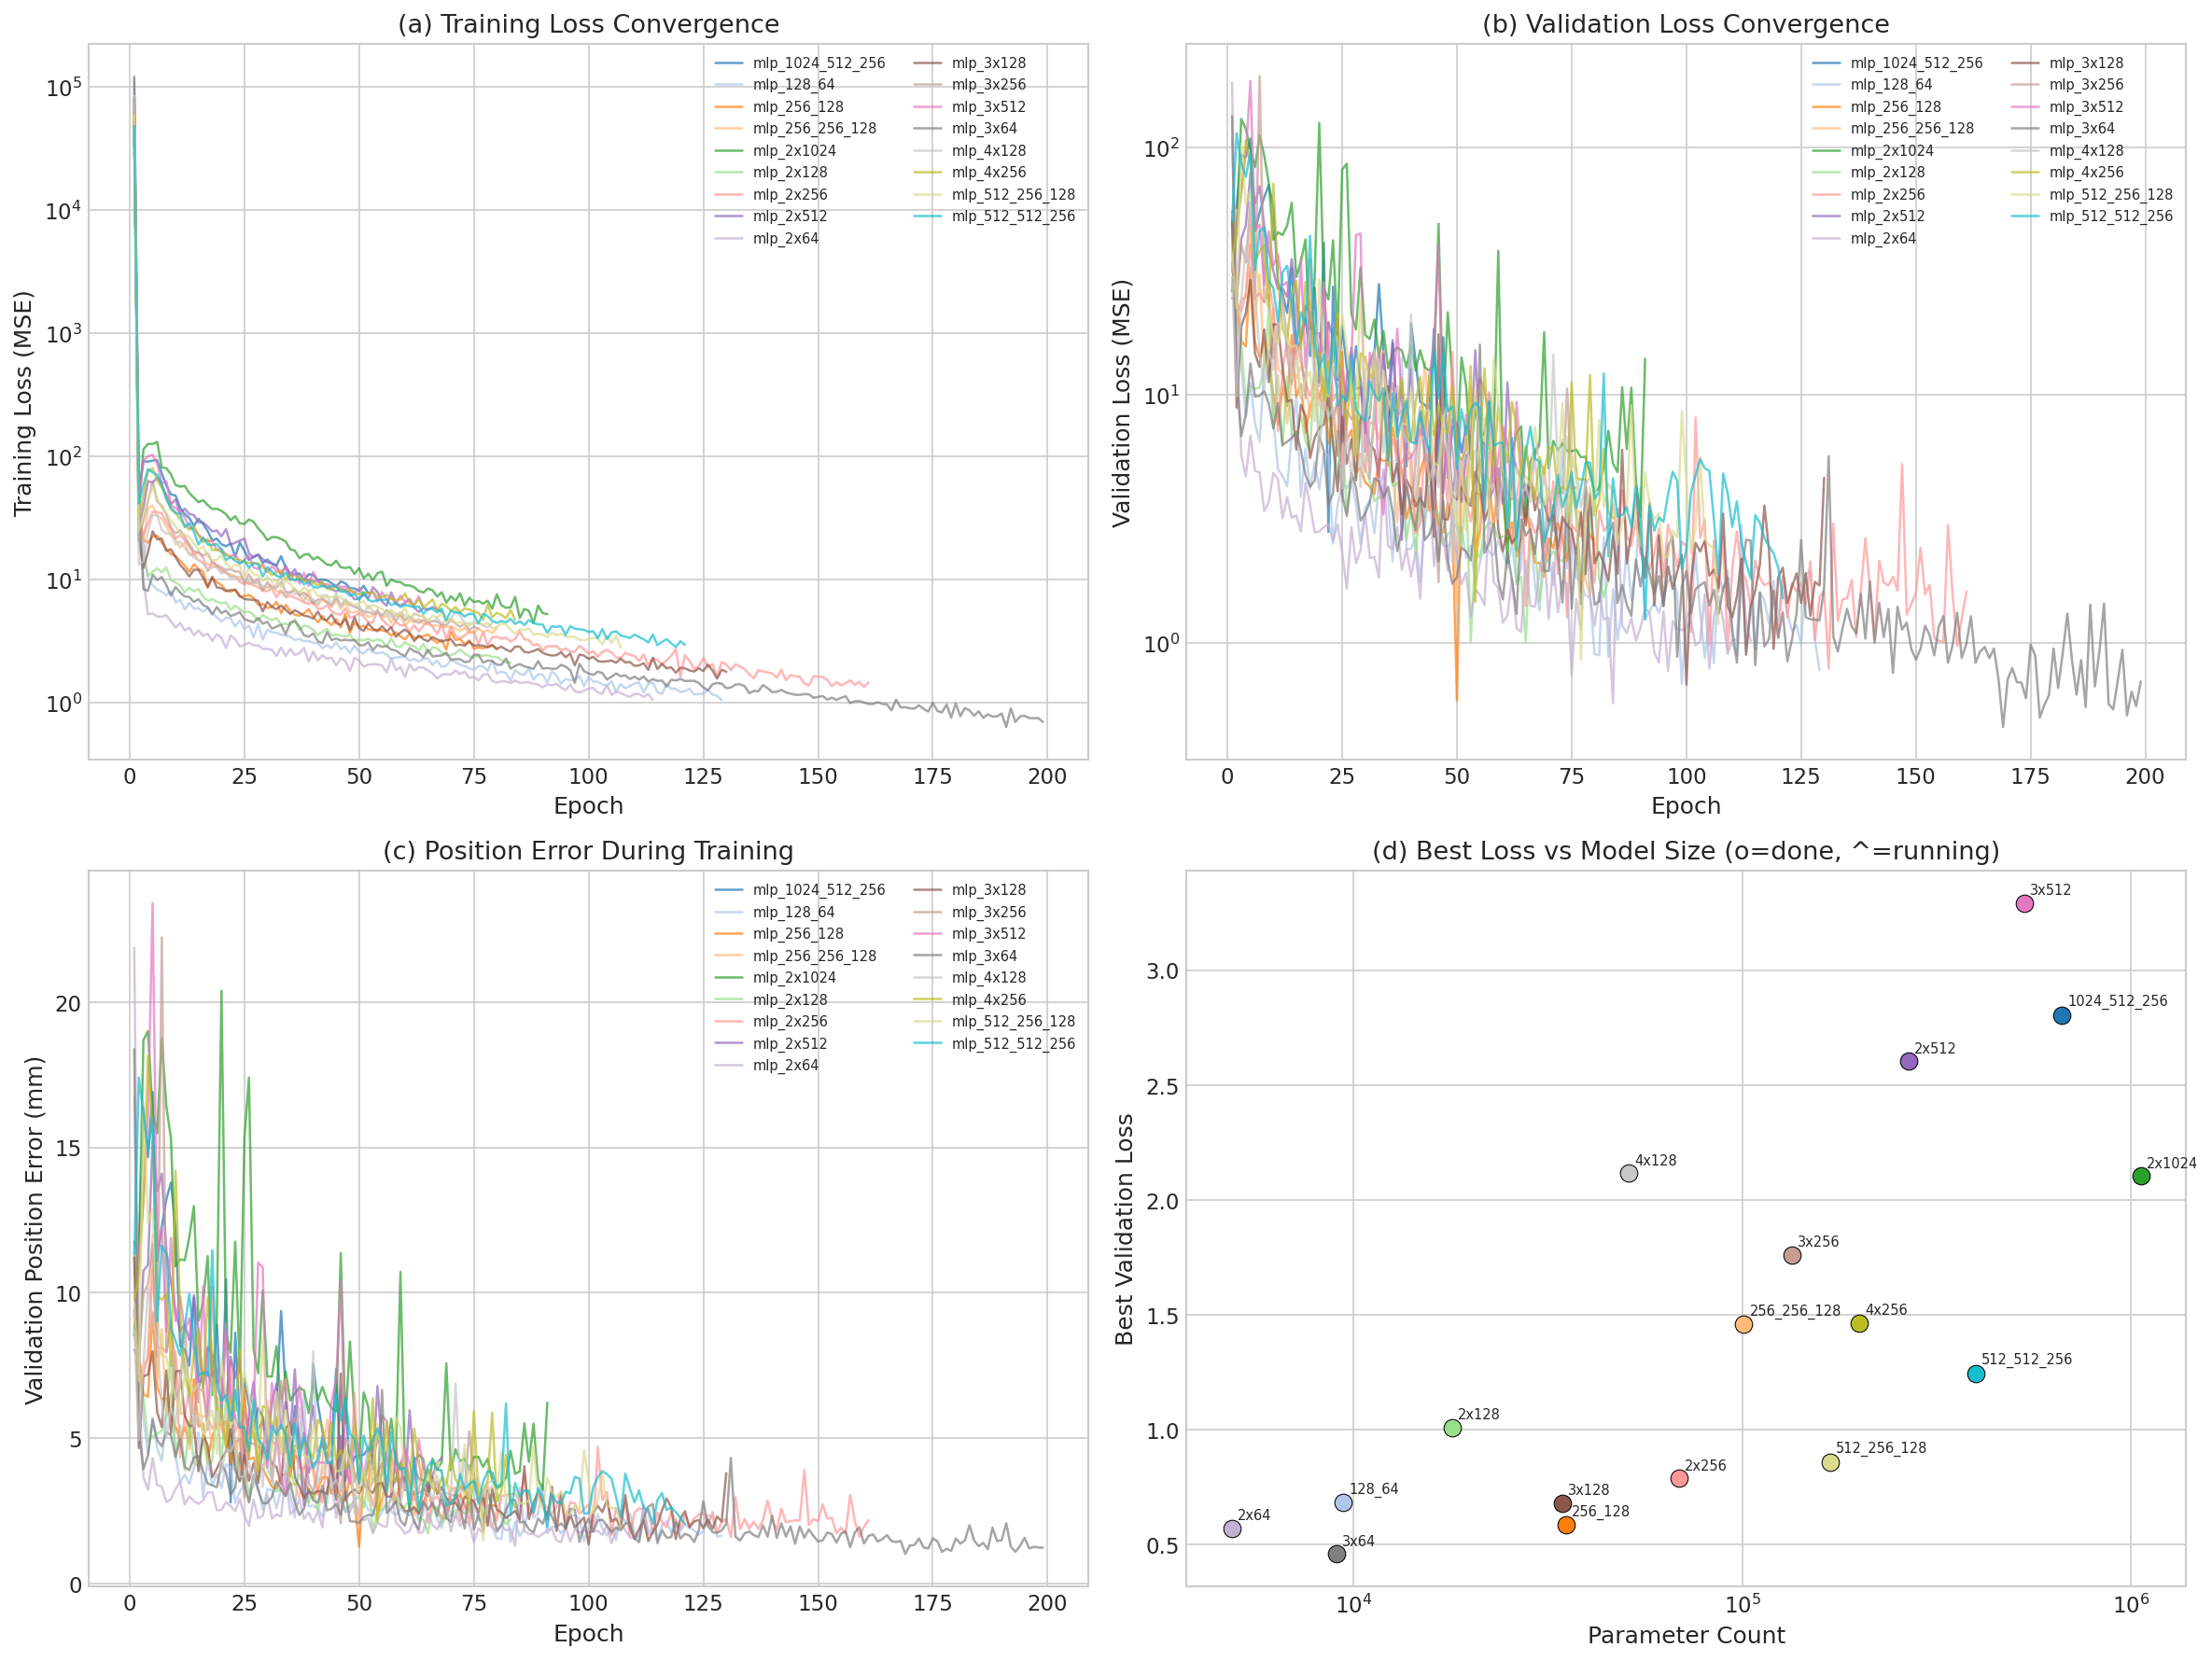
\includegraphics[width=\textwidth]{convergence_analysis.png}
\caption{Training and validation loss curves for all V1 MLP architectures. All 17 models reached convergence via early stopping.}
\label{fig:convergence}
\end{figure}

Figure~\ref{fig:diagnostics} provides additional training diagnostics including learning rate schedules and gradient norms.

\begin{figure}[H]
\centering
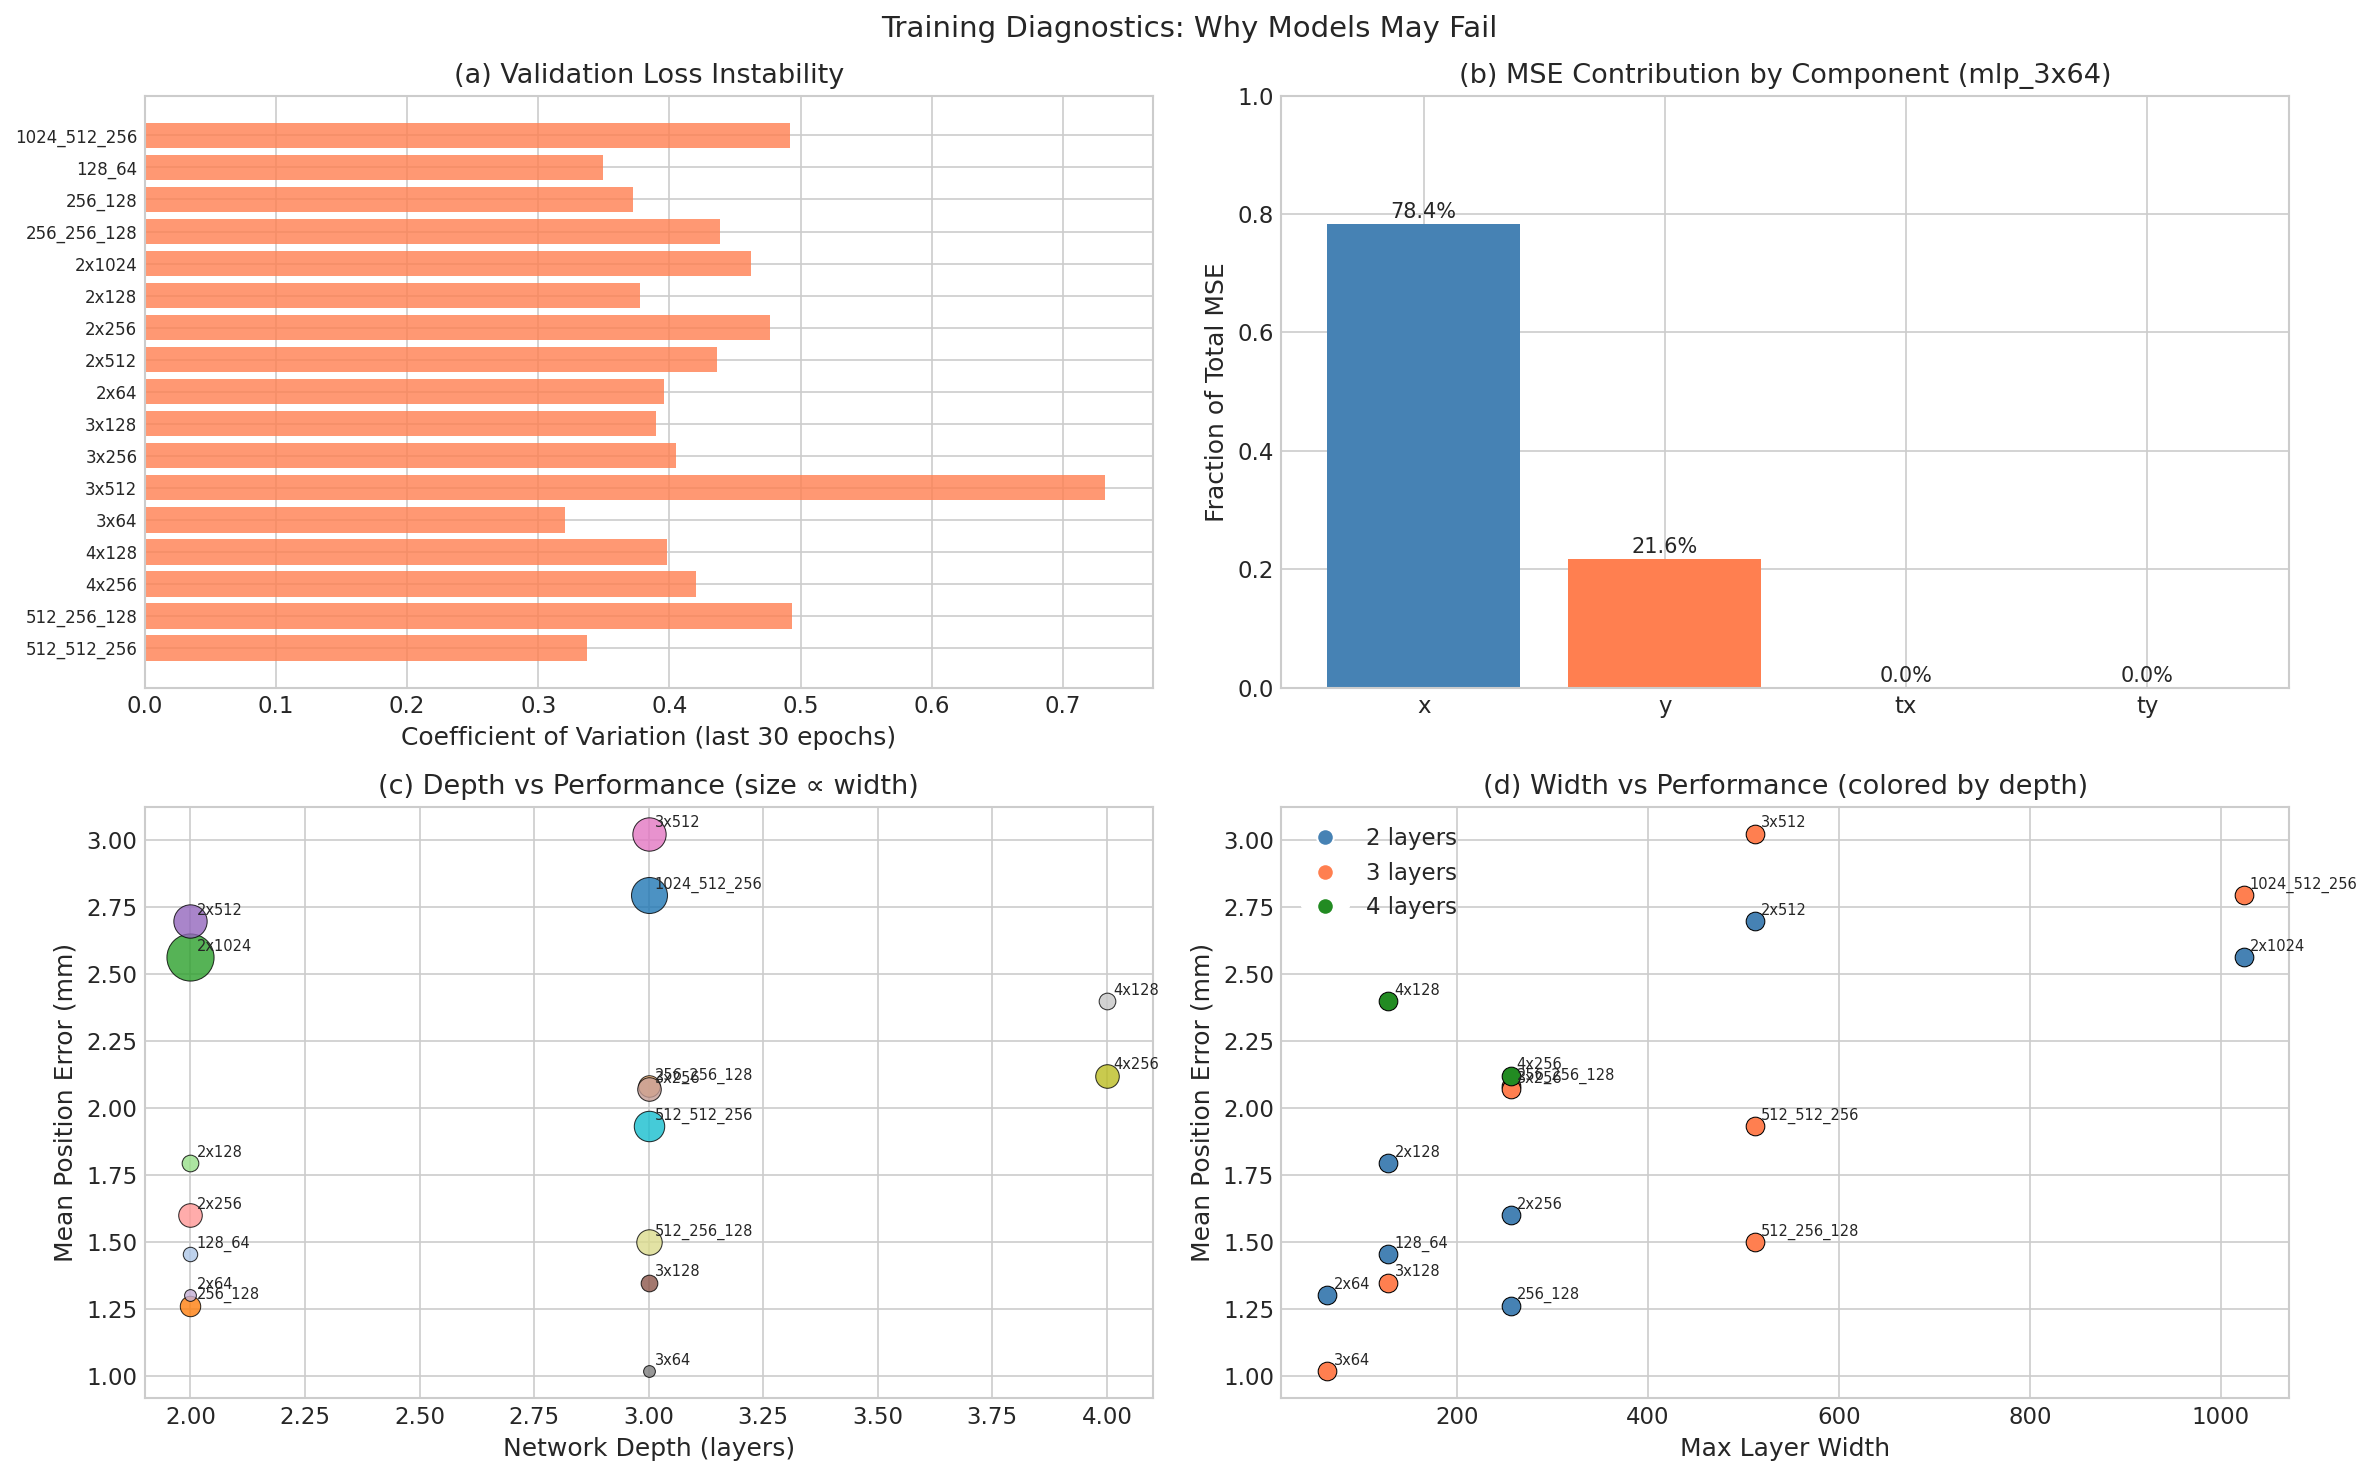
\includegraphics[width=\textwidth]{training_diagnostics.png}
\caption{Training diagnostics: learning rate schedules and gradient norm evolution across epochs.}
\label{fig:diagnostics}
\end{figure}

\subsection{Model Rankings}
\label{sec:rankings}

Table~\ref{tab:all_models} ranks all 17 models by mean position error on the 500K test set.

\begin{table}[H]
\centering
\caption{Performance of all V1 MLP models, ranked by mean position error. Position errors in mm; slope errors are dimensionless.}
\label{tab:all_models}
\begin{tabular}{@{}l r r r r r r r@{}}
\toprule
Model & Layers & Params & Pos.\ mean & Pos.\ 95\% & Pos.\ 99\% & $|\tx|$ MAE & $|\ty|$ MAE \\
      &        &        & (mm)       & (mm)       & (mm)       &               &               \\
\midrule
\texttt{mlp\_3x64}          & 3 &   9\,028 & 1.017 & 2.969 &  4.303 & 0.004041 & 0.004873 \\
\texttt{mlp\_256\_128}      & 2 &  35\,204 & 1.263 & 2.896 &  4.181 & 0.002319 & 0.002274 \\
\texttt{mlp\_2x64}          & 2 &   4\,868 & 1.302 & 2.630 &  3.573 & 0.001662 & 0.001633 \\
\texttt{mlp\_3x128}         & 3 &  34\,436 & 1.349 & 3.242 &  4.944 & 0.002441 & 0.002423 \\
\texttt{mlp\_128\_64}       & 2 &   9\,412 & 1.455 & 2.897 &  3.866 & 0.002845 & 0.002234 \\
\texttt{mlp\_512\_256\_128} & 3 & 168\,324 & 1.499 & 3.599 &  5.611 & 0.003355 & 0.003319 \\
\texttt{mlp\_2x256}         & 2 &  68\,612 & 1.601 & 2.954 &  3.509 & 0.001858 & 0.001363 \\
\texttt{mlp\_2x128}         & 2 &  17\,924 & 1.793 & 3.417 &  4.462 & 0.001567 & 0.001480 \\
\texttt{mlp\_512\_512\_256} & 3 & 398\,596 & 1.934 & 3.987 &  5.220 & 0.003418 & 0.002534 \\
\texttt{mlp\_3x256}         & 3 & 134\,404 & 2.071 & 5.568 &  7.760 & 0.002595 & 0.002500 \\
\texttt{mlp\_256\_256\_128} & 3 & 100\,996 & 2.083 & 4.413 &  6.148 & 0.004859 & 0.003643 \\
\texttt{mlp\_4x256}         & 4 & 200\,196 & 2.121 & 4.232 &  5.386 & 0.003433 & 0.003260 \\
\texttt{mlp\_4x128}         & 4 &  50\,948 & 2.400 & 5.728 &  8.478 & 0.004519 & 0.005875 \\
\texttt{mlp\_2x1024}        & 2 & 1\,060\,868 & 2.562 & 5.055 & 6.727 & 0.002207 & 0.002017 \\
\texttt{mlp\_2x512}         & 2 & 268\,292 & 2.697 & 5.887 &  9.273 & 0.001654 & 0.001833 \\
\texttt{mlp\_1024\_512\_256}& 3 & 664\,324 & 2.796 & 6.101 &  9.522 & 0.002769 & 0.002050 \\
\texttt{mlp\_3x512}         & 3 & 530\,948 & 3.024 & 6.569 &  9.603 & 0.002870 & 0.002574 \\
\bottomrule
\end{tabular}
\end{table}

\subsection{Key Observations}

\begin{enumerate}[nosep]
  \item \textbf{Small models win}: The best model (\texttt{mlp\_3x64}, 3 layers, 9K params) outperforms all larger architectures.
  The top 5 models all have $\leq$\,35K parameters, with \texttt{mlp\_2x64} (4\,868 params) ranking third.

  \item \textbf{Diminishing returns from width}: Increasing layer width beyond 128 neurons provides no benefit and often degrades performance.
  The 4-layer and wide 512/1024-class models consistently rank in the bottom half.

  \item \textbf{Over-parameterisation does not help}: \texttt{mlp\_2x1024} (1.06M params) performs worse than \texttt{mlp\_3x64} (9K params), confirming the bottleneck is the loss function, not model capacity.

  \item \textbf{x--y asymmetry}: All models show $|x\text{ error}| \gg |y\text{ error}|$, reflecting the dominant $B_y$ field component that drives bending in the $x$--$z$ plane.
\end{enumerate}

Figure~\ref{fig:model_heatmap} compares all models across the key error metrics as a heatmap.

\begin{figure}[H]
\centering
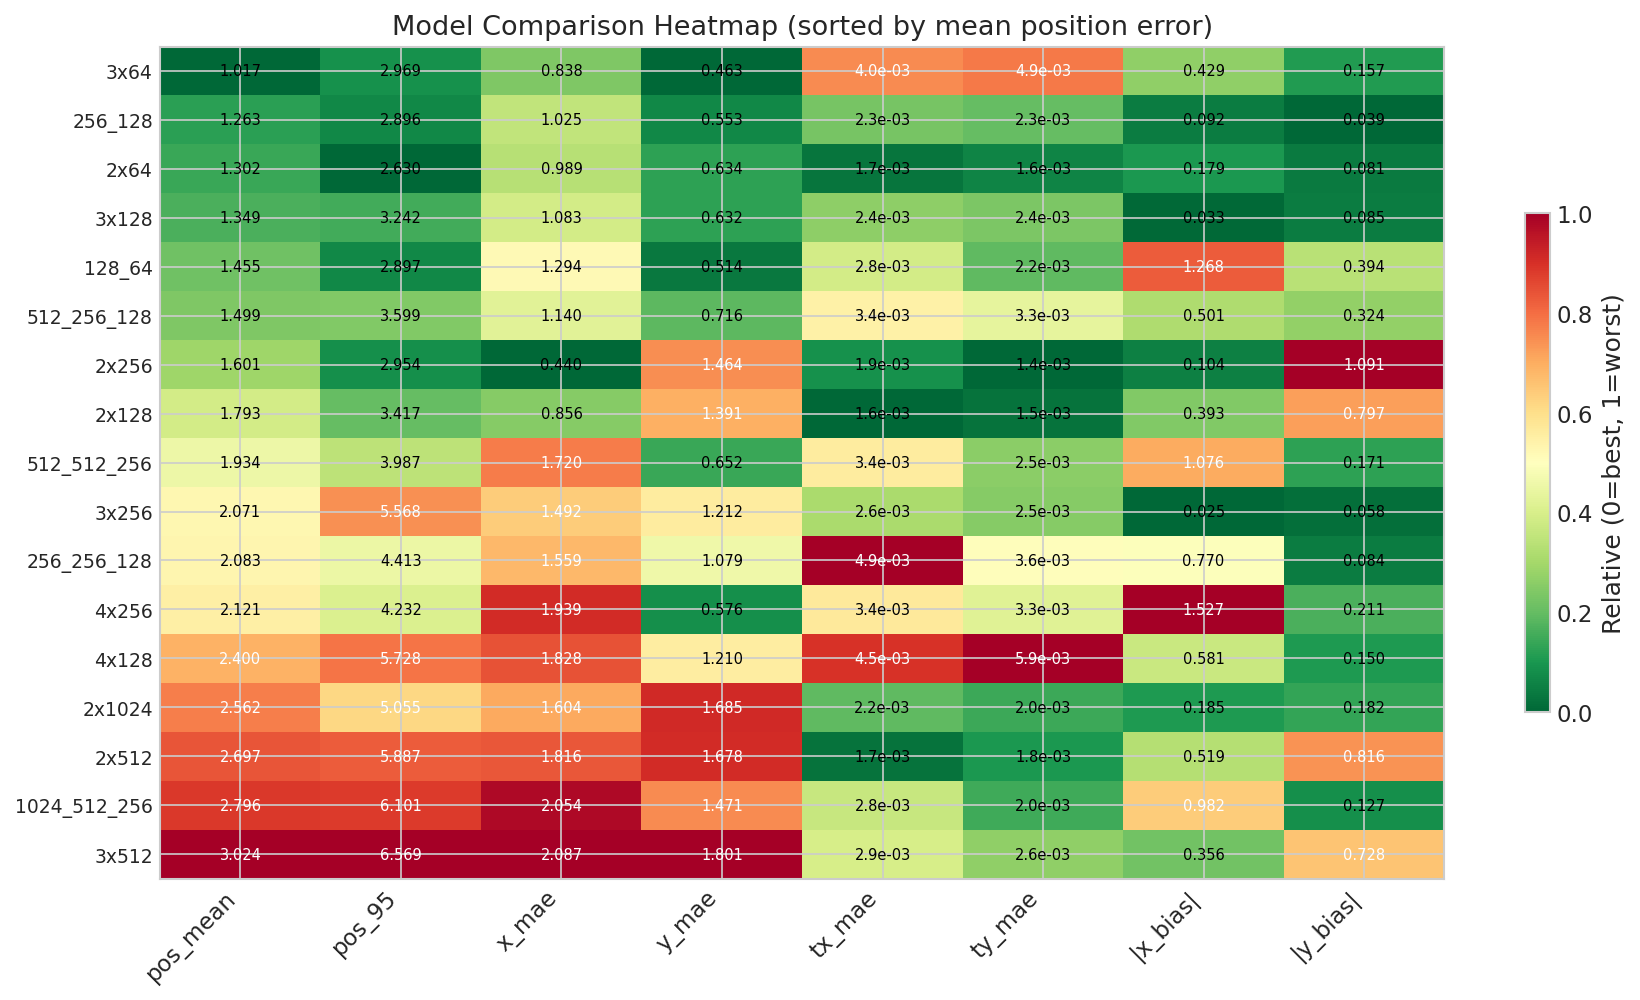
\includegraphics[width=\textwidth]{model_comparison_heatmap.png}
\caption{Multi-model comparison heatmap showing position and slope errors across all 17 architectures.}
\label{fig:model_heatmap}
\end{figure}

%=============================================================================
\section{Diagnostic Analysis: Why V1 Performance Saturates}
\label{sec:diagnostics}

\subsection{MSE Contribution Breakdown}

For the best model (\texttt{mlp\_3x64}), the contribution of each output component to the total MSE loss is:
\begin{equation}
  \text{MSE}_x : \text{MSE}_y : \text{MSE}_{\tx} : \text{MSE}_{\ty} \;=\; 78.4\% : 21.6\% : 0.0\% : 0.0\%
\end{equation}
The slopes $\tx$ and $\ty$ contribute \emph{negligibly} to the total loss.
This means the optimiser effectively ignores bending physics --- the model learns only the kinematic mapping $x' \approx x + \tx \cdot \dz$ and does not invest capacity in the field-driven slope changes $\Delta\tx$ and $\Delta\ty$.

\subsection{Target Dynamic Range}
\label{sec:dynamic_range}

The root cause is the extreme dynamic range between output components (Table~\ref{tab:dynamic_range}).

\begin{table}[H]
\centering
\caption{Standard deviation of raw output targets vs.\ residual (field-driven) targets, showing the compression ratio. The residual formulation removes the dominant kinematic term.}
\label{tab:dynamic_range}
\begin{tabular}{@{}l r r r@{}}
\toprule
Component & Raw $\sigma$ & Residual $\sigma$ & Compression \\
\midrule
$x_\text{out}$\,/\,$\delta x_\text{field}$ & 827.1564 & 0.8397 & $985\times$ \\
$y_\text{out}$\,/\,$\delta y_\text{field}$ & 689.9211 & 0.0868 & $7951\times$ \\
$\tx'$\,/\,$\Delta\tx$                      & 0.1733   & 0.000189 & $919\times$ \\
$\ty'$\,/\,$\Delta\ty$                      & 0.1444   & 0.0000255 & $5656\times$ \\
\bottomrule
\end{tabular}
\end{table}

The raw $x_\text{out}$ has standard deviation $\sigma = 827$\,mm, while the field-driven deflection $\delta x = x' - (x + \tx \cdot \dz)$ has $\sigma = 0.84$\,mm --- a compression of $985\times$.
The model wastes the vast majority of its capacity learning the trivial linear kinematic term.

Figure~\ref{fig:xy_asymmetry} visualises the $x$--$y$ deflection asymmetry and its connection to the dipole field structure.

\begin{figure}[H]
\centering
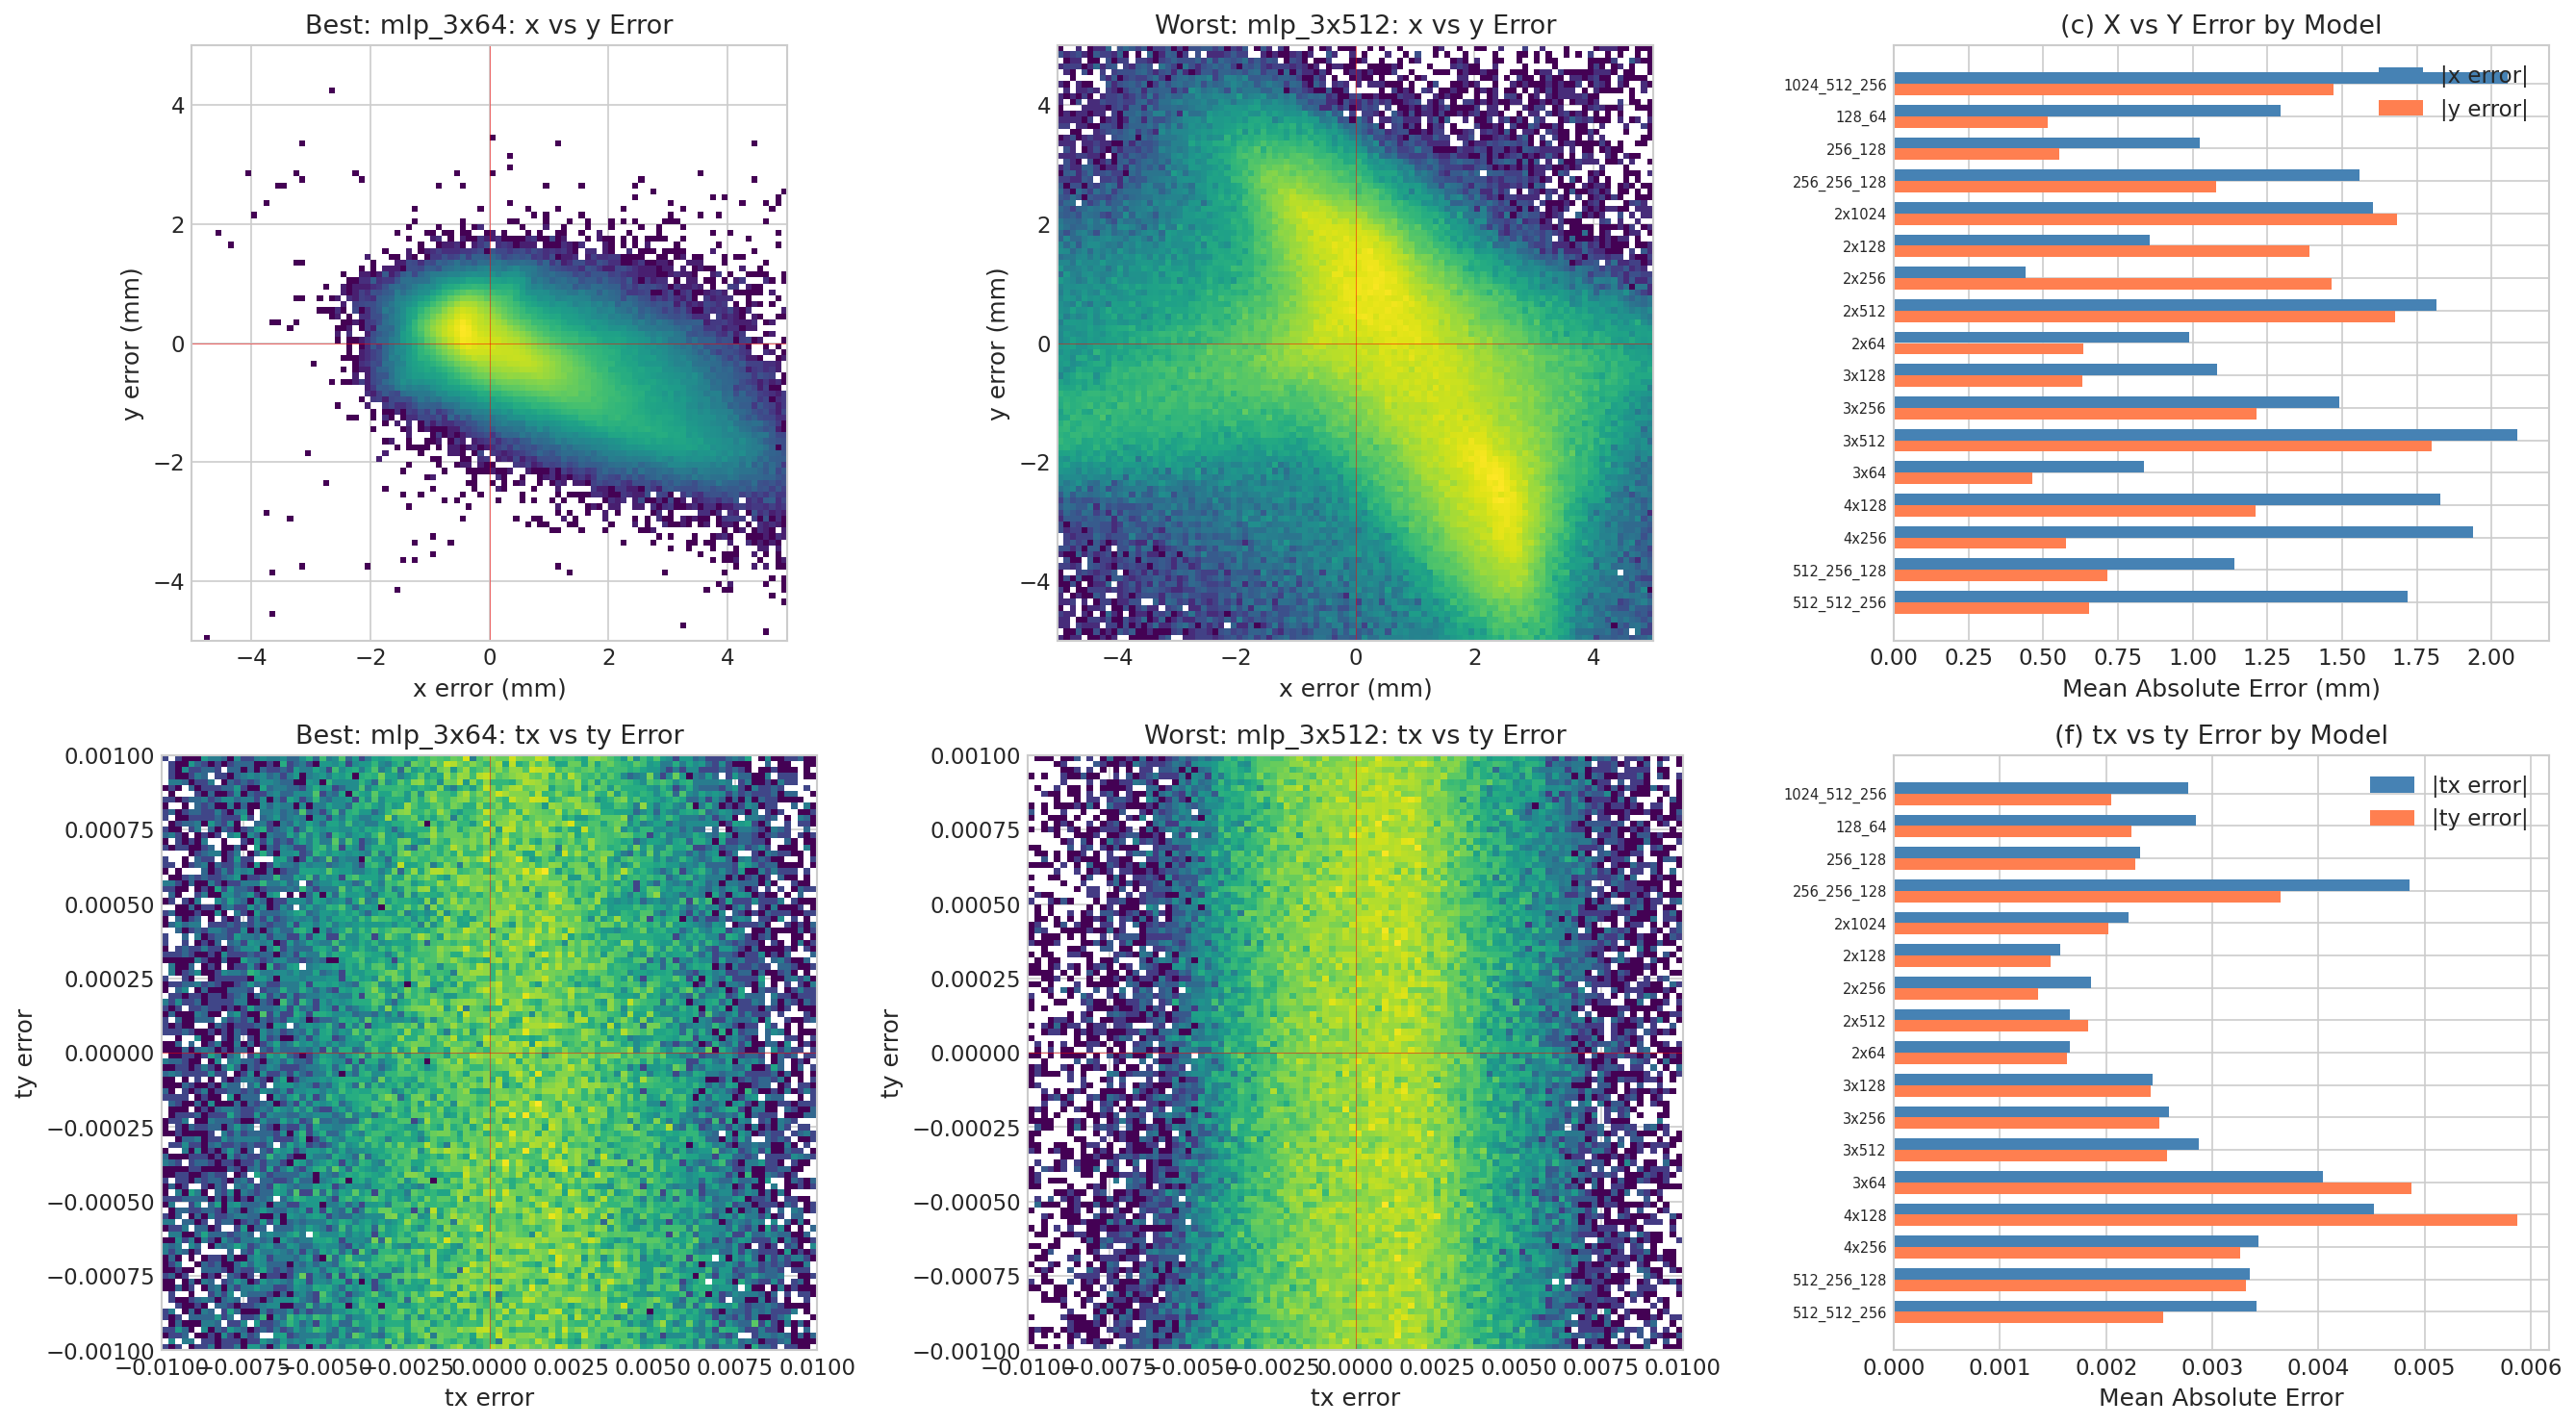
\includegraphics[width=\textwidth]{xy_deflection_asymmetry.png}
\caption{Position error asymmetry between $x$ (bending plane) and $y$ (non-bending plane) for the best model. The $x$ deflection is an order of magnitude larger, reflecting the dominant $B_y$ component.}
\label{fig:xy_asymmetry}
\end{figure}

\subsection{Momentum Dependence}

Table~\ref{tab:p_bins} shows the residual target standard deviations by momentum bin.
Low-momentum tracks ($p < 2$\,GeV) have $\sim\!27\times$ larger $\sigma(\delta x)$ than high-momentum tracks ($p > 20$\,GeV).
The log-uniform sampling ensures equal representation, but the variance-dominated loss still focuses on low-$p$ tracks.

\begin{table}[H]
\centering
\caption{Residual target statistics by momentum bin (500K test samples). Deflections scale as $\Delta\tx \propto \qop$, so low-$p$ tracks dominate the variance.}
\label{tab:p_bins}
\begin{tabular}{@{}l r r r r r@{}}
\toprule
Momentum bin & $N$ & $\sigma(\delta x)$ & $\sigma(\delta y)$ & $\sigma(\Delta\tx)$ & $\sigma(\Delta\ty)$ \\
             &     & (mm)               & (mm)               &                       &                       \\
\midrule
1--2\,GeV   &  75\,283 & 1.8741 & 0.1942 & 0.000421 & 0.000057 \\
2--5\,GeV   &  99\,466 & 0.8616 & 0.0880 & 0.000193 & 0.000026 \\
5--20\,GeV  & 151\,140 & 0.2985 & 0.0310 & 0.000067 & 0.000009 \\
20--100\,GeV& 174\,111 & 0.0702 & 0.0073 & 0.000016 & 0.000002 \\
\bottomrule
\end{tabular}
\end{table}

Figure~\ref{fig:error_vs_p} shows the error dependence on momentum, confirming the expected $1/p$ scaling.

\begin{figure}[H]
\centering
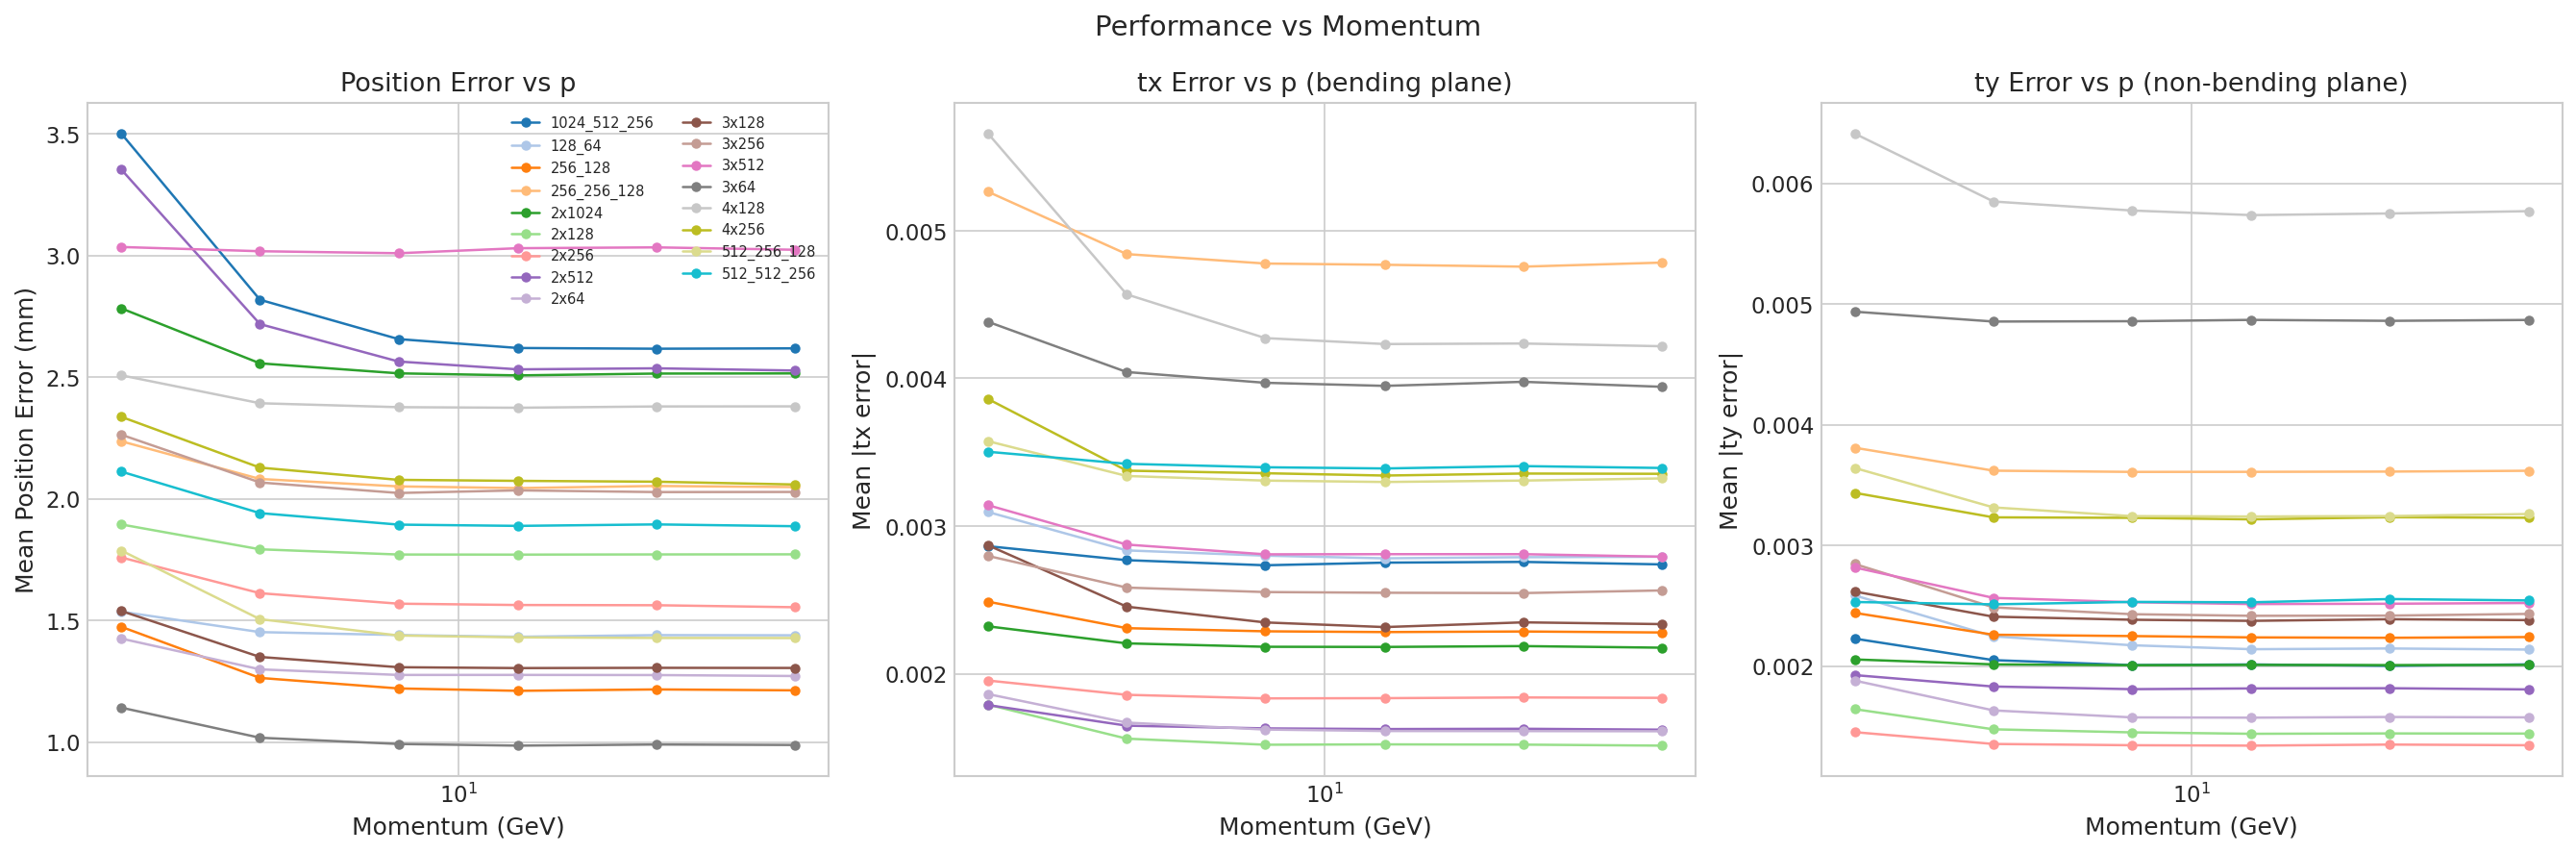
\includegraphics[width=\textwidth]{error_vs_momentum.png}
\caption{Position and slope errors as a function of track momentum. Low-momentum tracks ($p < 5$\,GeV) show significantly larger errors due to stronger field-driven deflection.}
\label{fig:error_vs_p}
\end{figure}

\subsection{Spatial Dependence}

Figures~\ref{fig:error_vs_state}--\ref{fig:error_heatmap} show the error dependence on initial track state parameters and the $(z, \dz)$ phase space.

\begin{figure}[H]
\centering
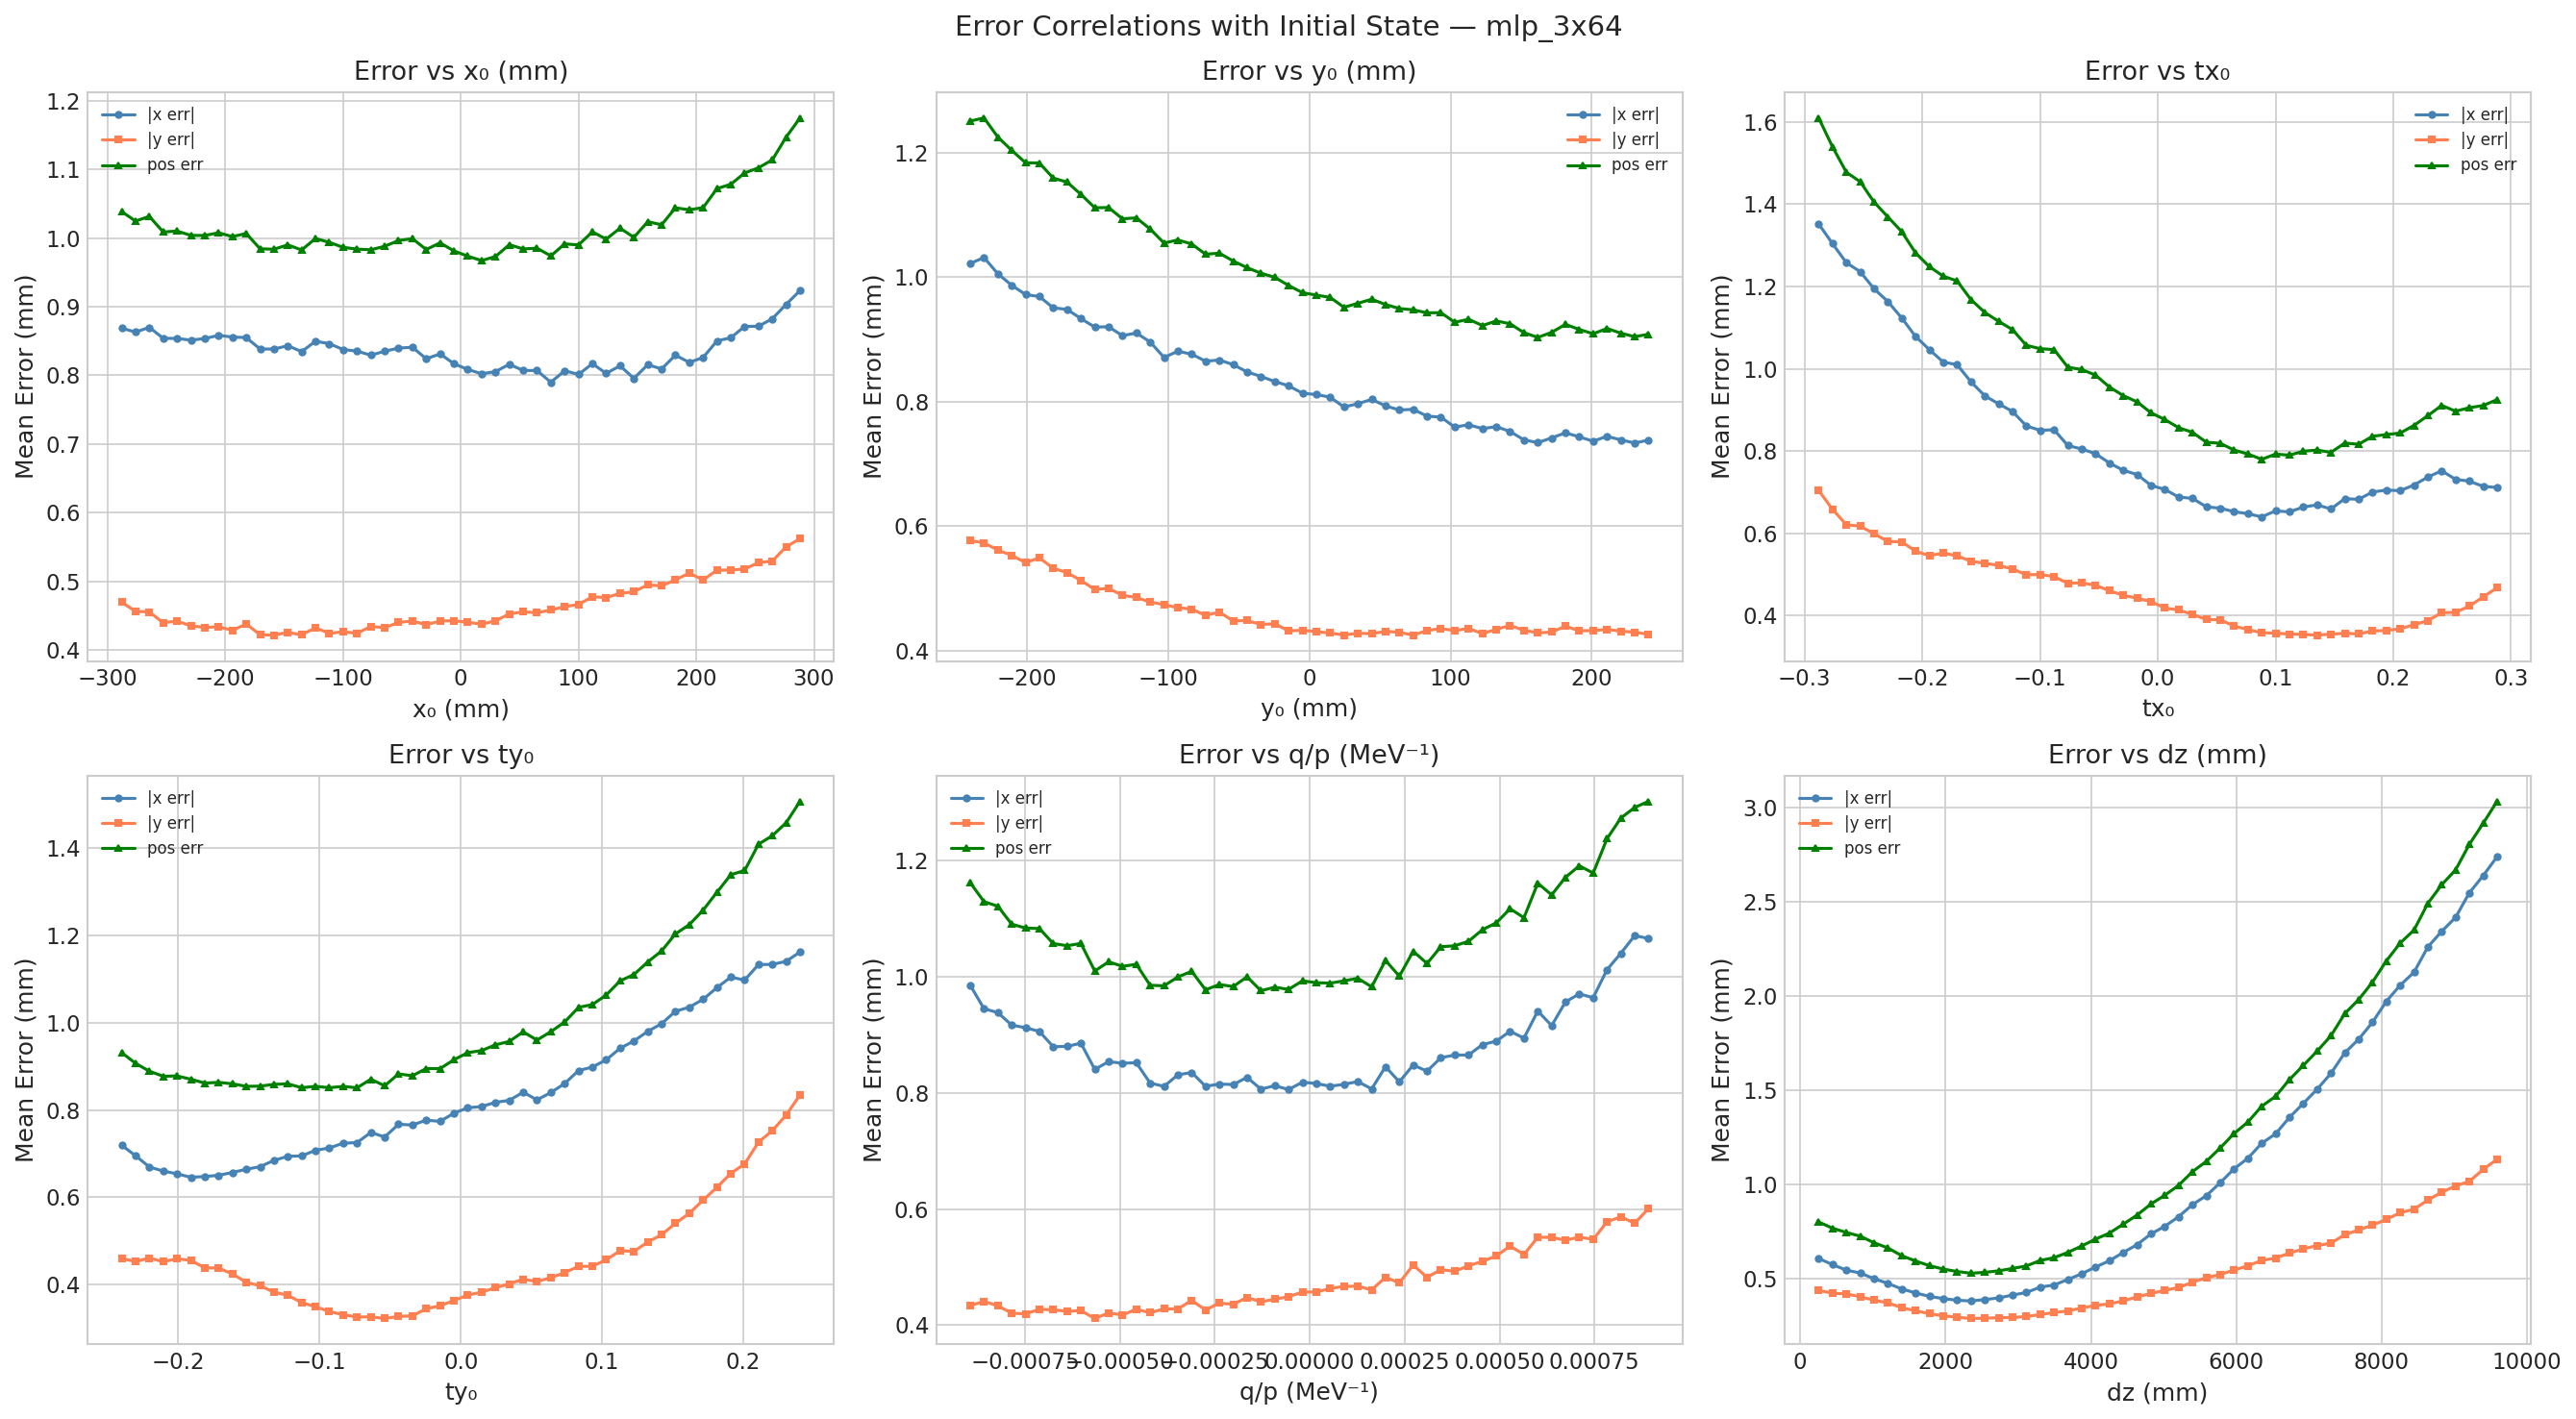
\includegraphics[width=\textwidth]{error_vs_initial_state.png}
\caption{Position error as a function of initial track state parameters ($x$, $y$, $\tx$, $\ty$, $\qop$, $\dz$).}
\label{fig:error_vs_state}
\end{figure}

\begin{figure}[H]
\centering
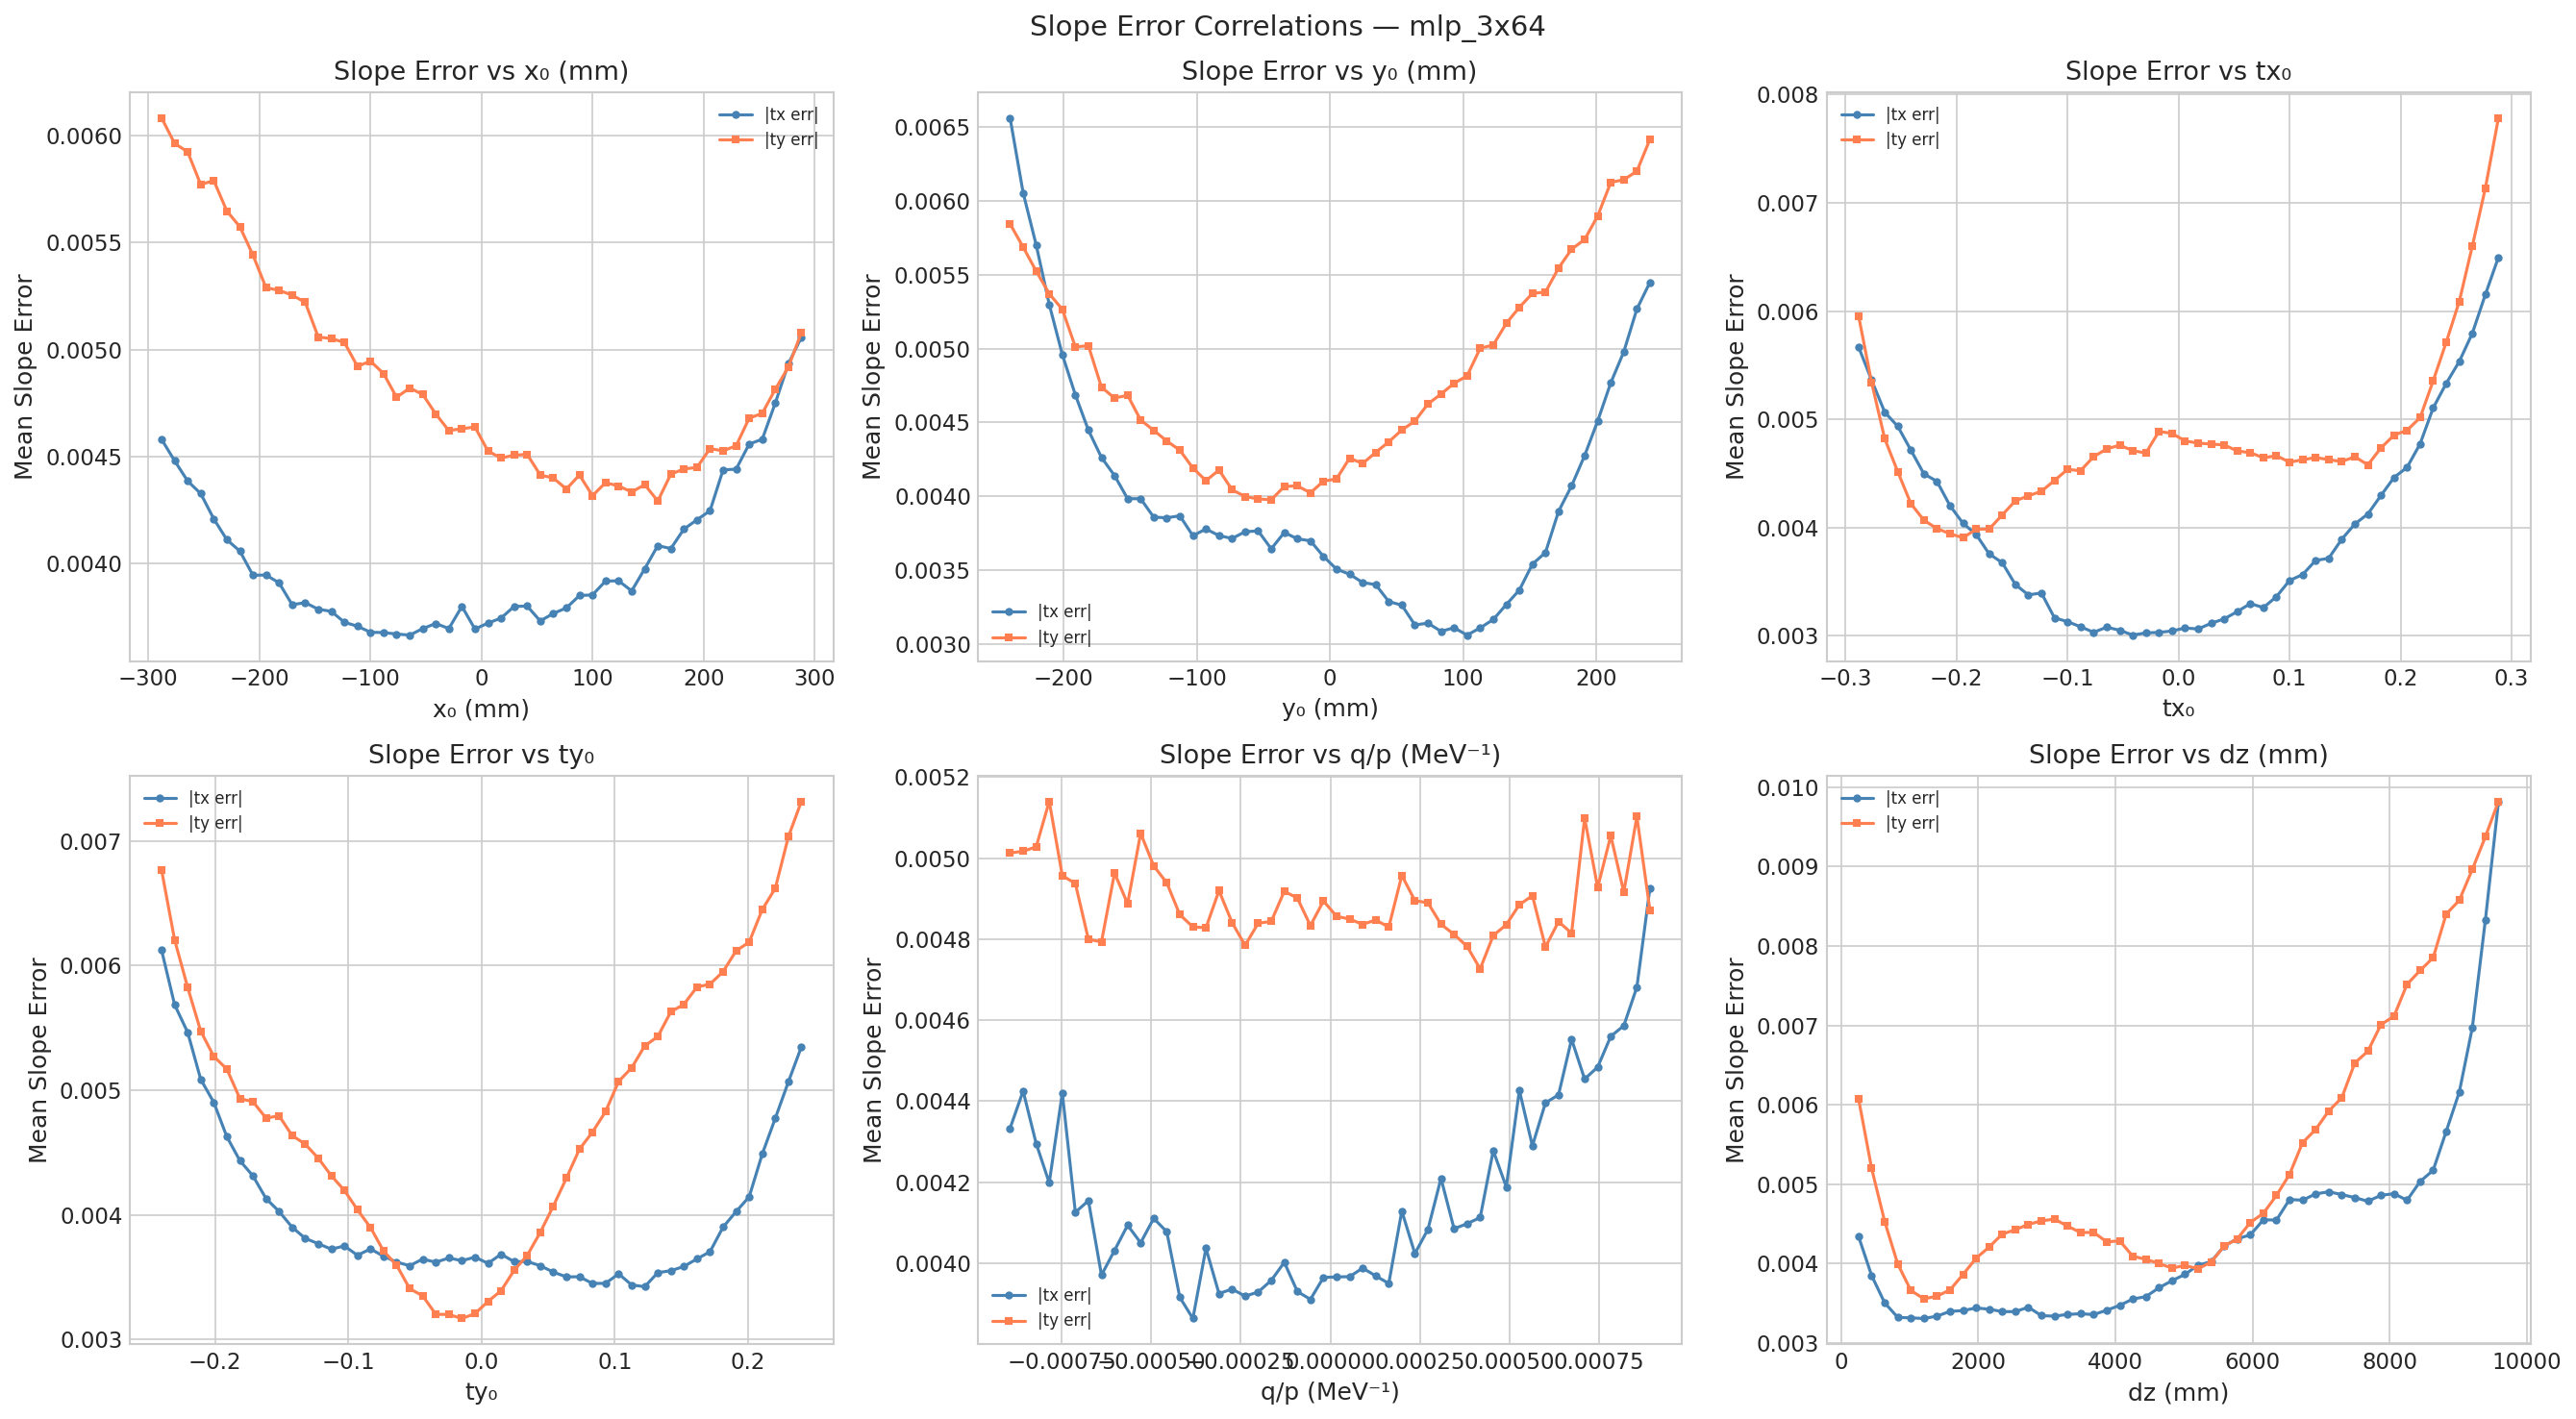
\includegraphics[width=\textwidth]{slope_error_vs_initial_state.png}
\caption{Slope error as a function of initial track state parameters.}
\label{fig:slope_error_vs_state}
\end{figure}

\begin{figure}[H]
\centering
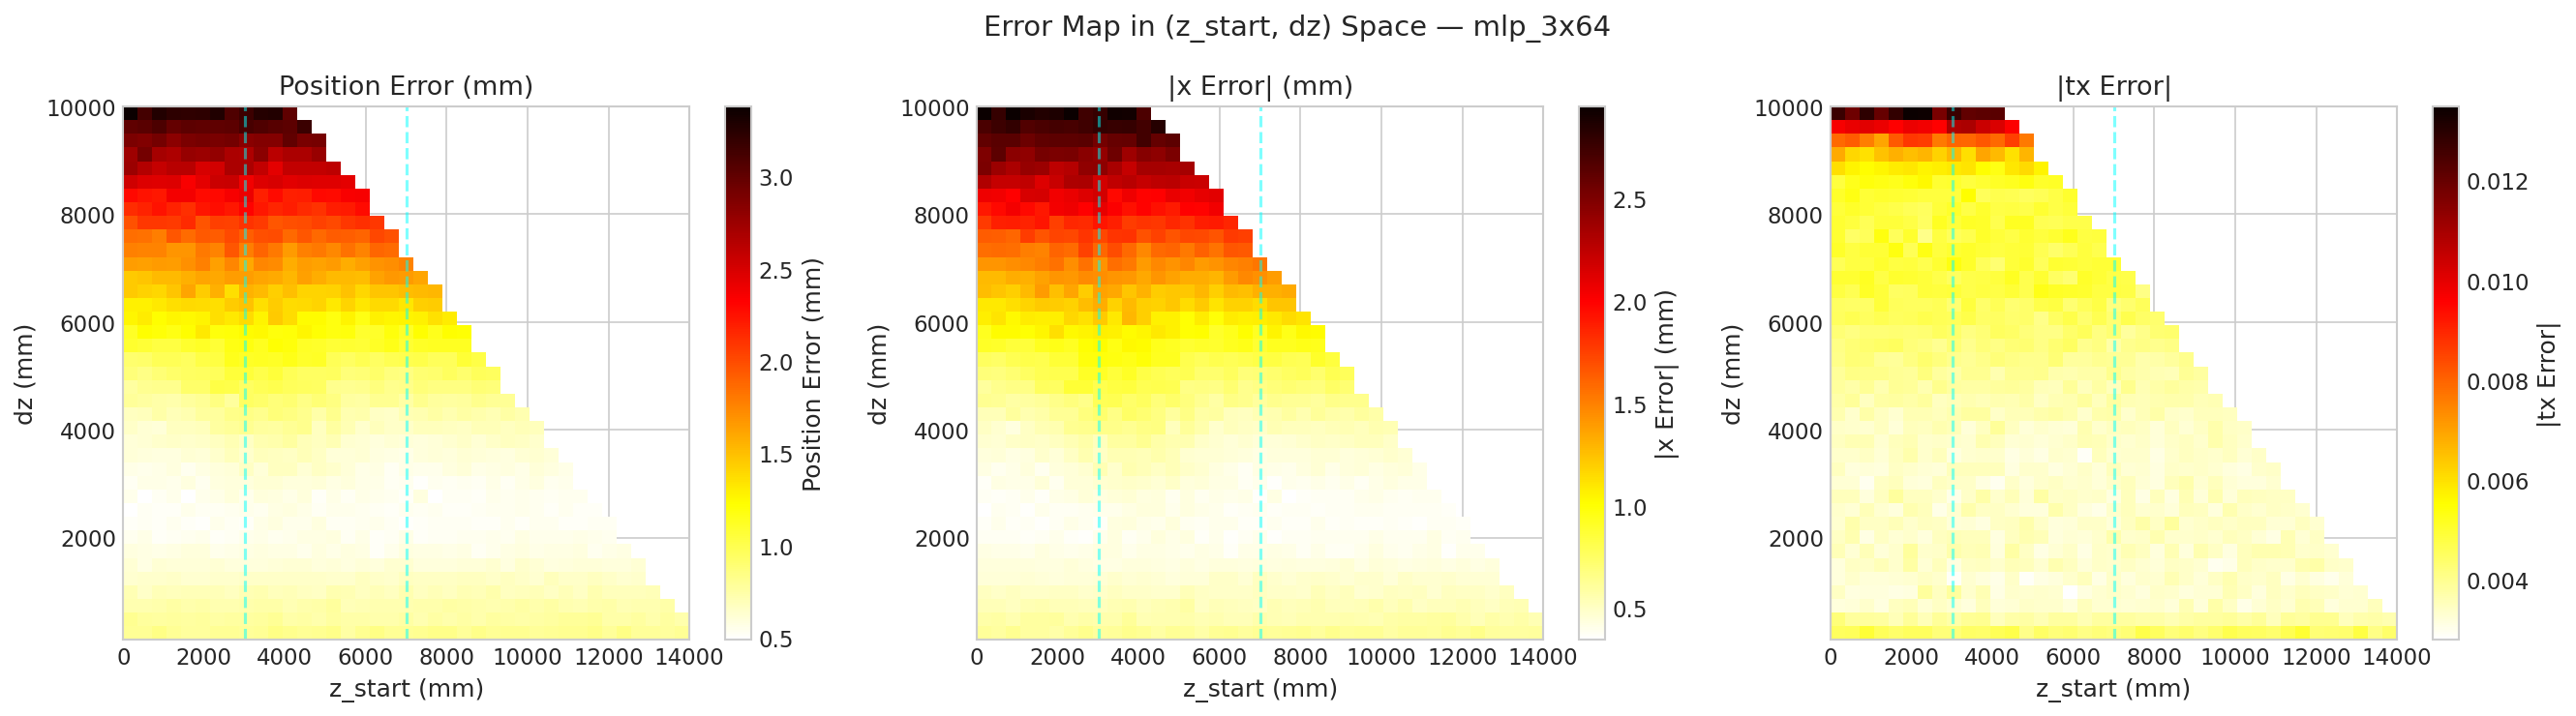
\includegraphics[width=\textwidth]{error_heatmap_z_dz.png}
\caption{Position error heatmap in the $(z_\text{start}, \dz)$ plane. The error is largest for long-range propagations through the field centre ($z \approx 5000$\,mm, field peak).}
\label{fig:error_heatmap}
\end{figure}

\begin{figure}[H]
\centering
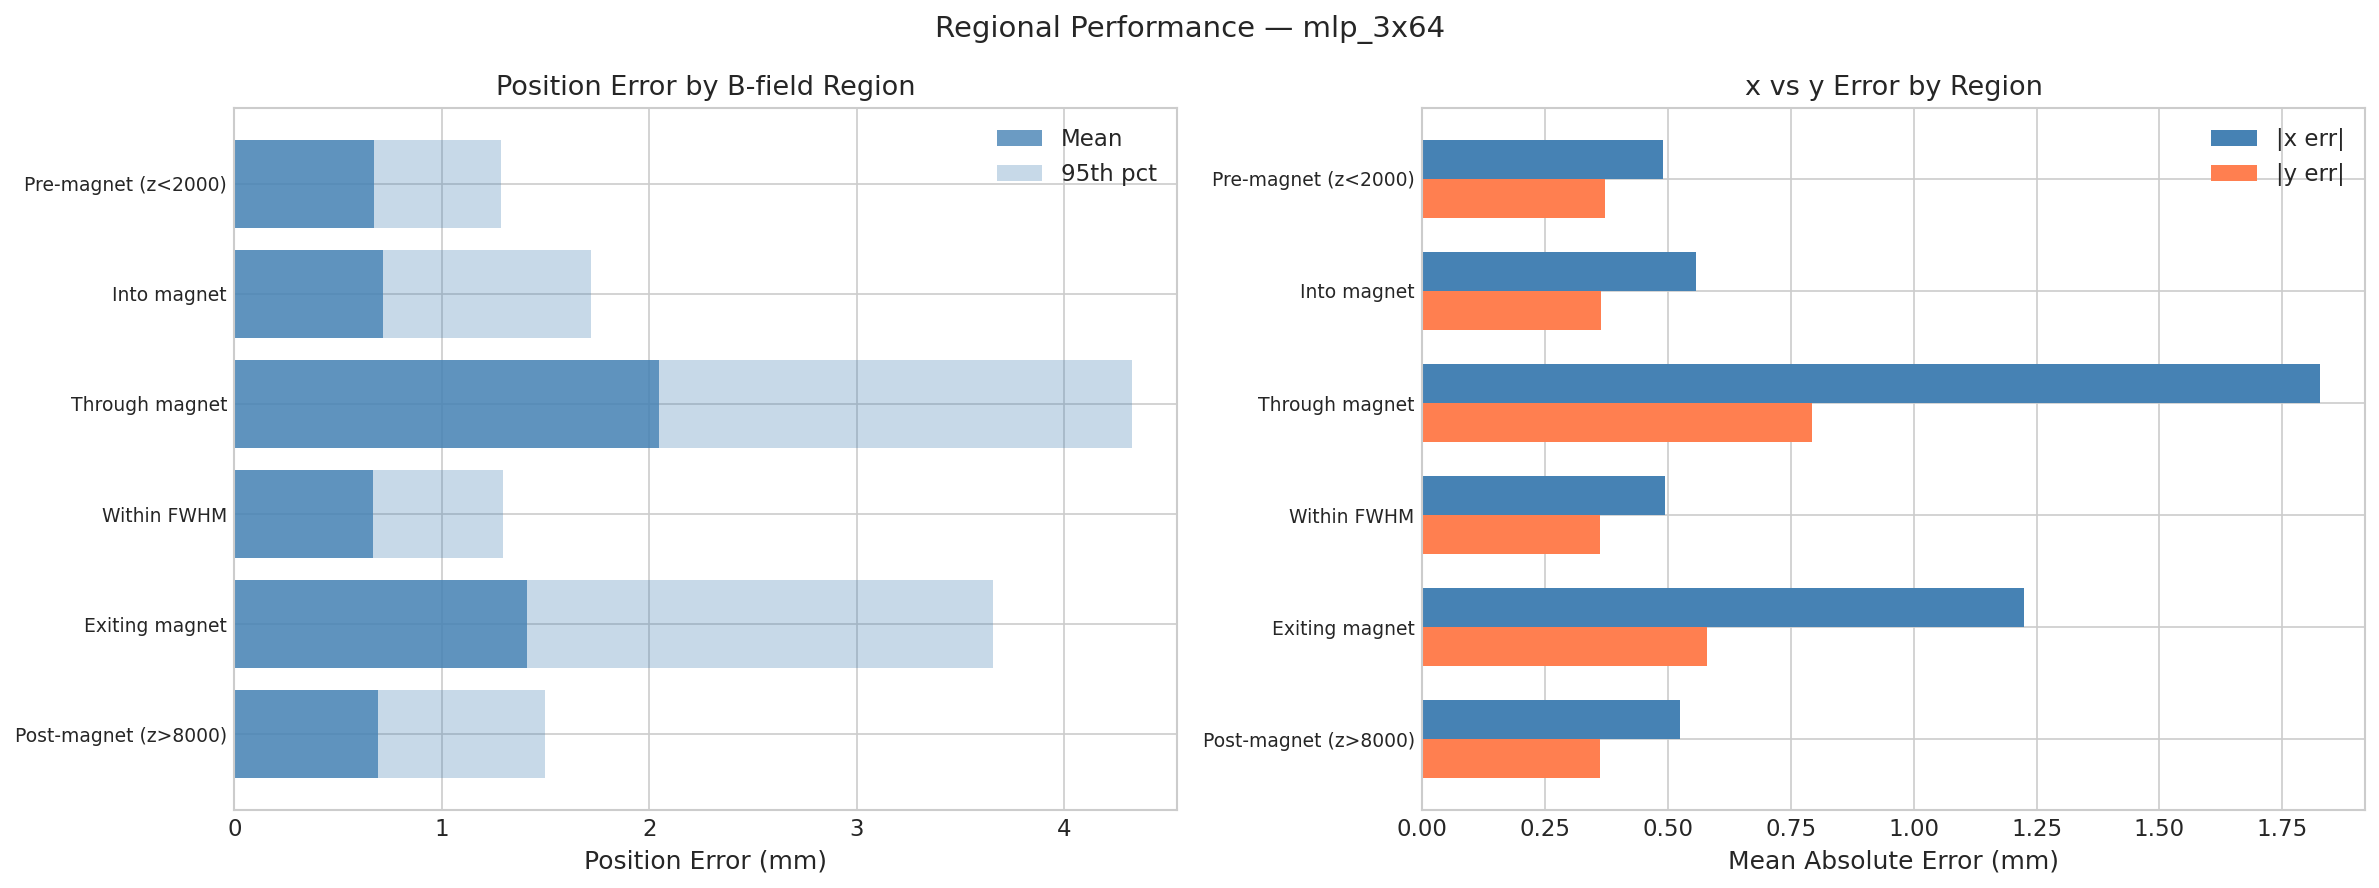
\includegraphics[width=\textwidth]{regional_performance.png}
\caption{Regional performance breakdown showing error variation across different detector regions.}
\label{fig:regional}
\end{figure}

\subsection{Error Distributions}

Figure~\ref{fig:error_dist} shows the full error distributions for the best model.

\begin{figure}[H]
\centering
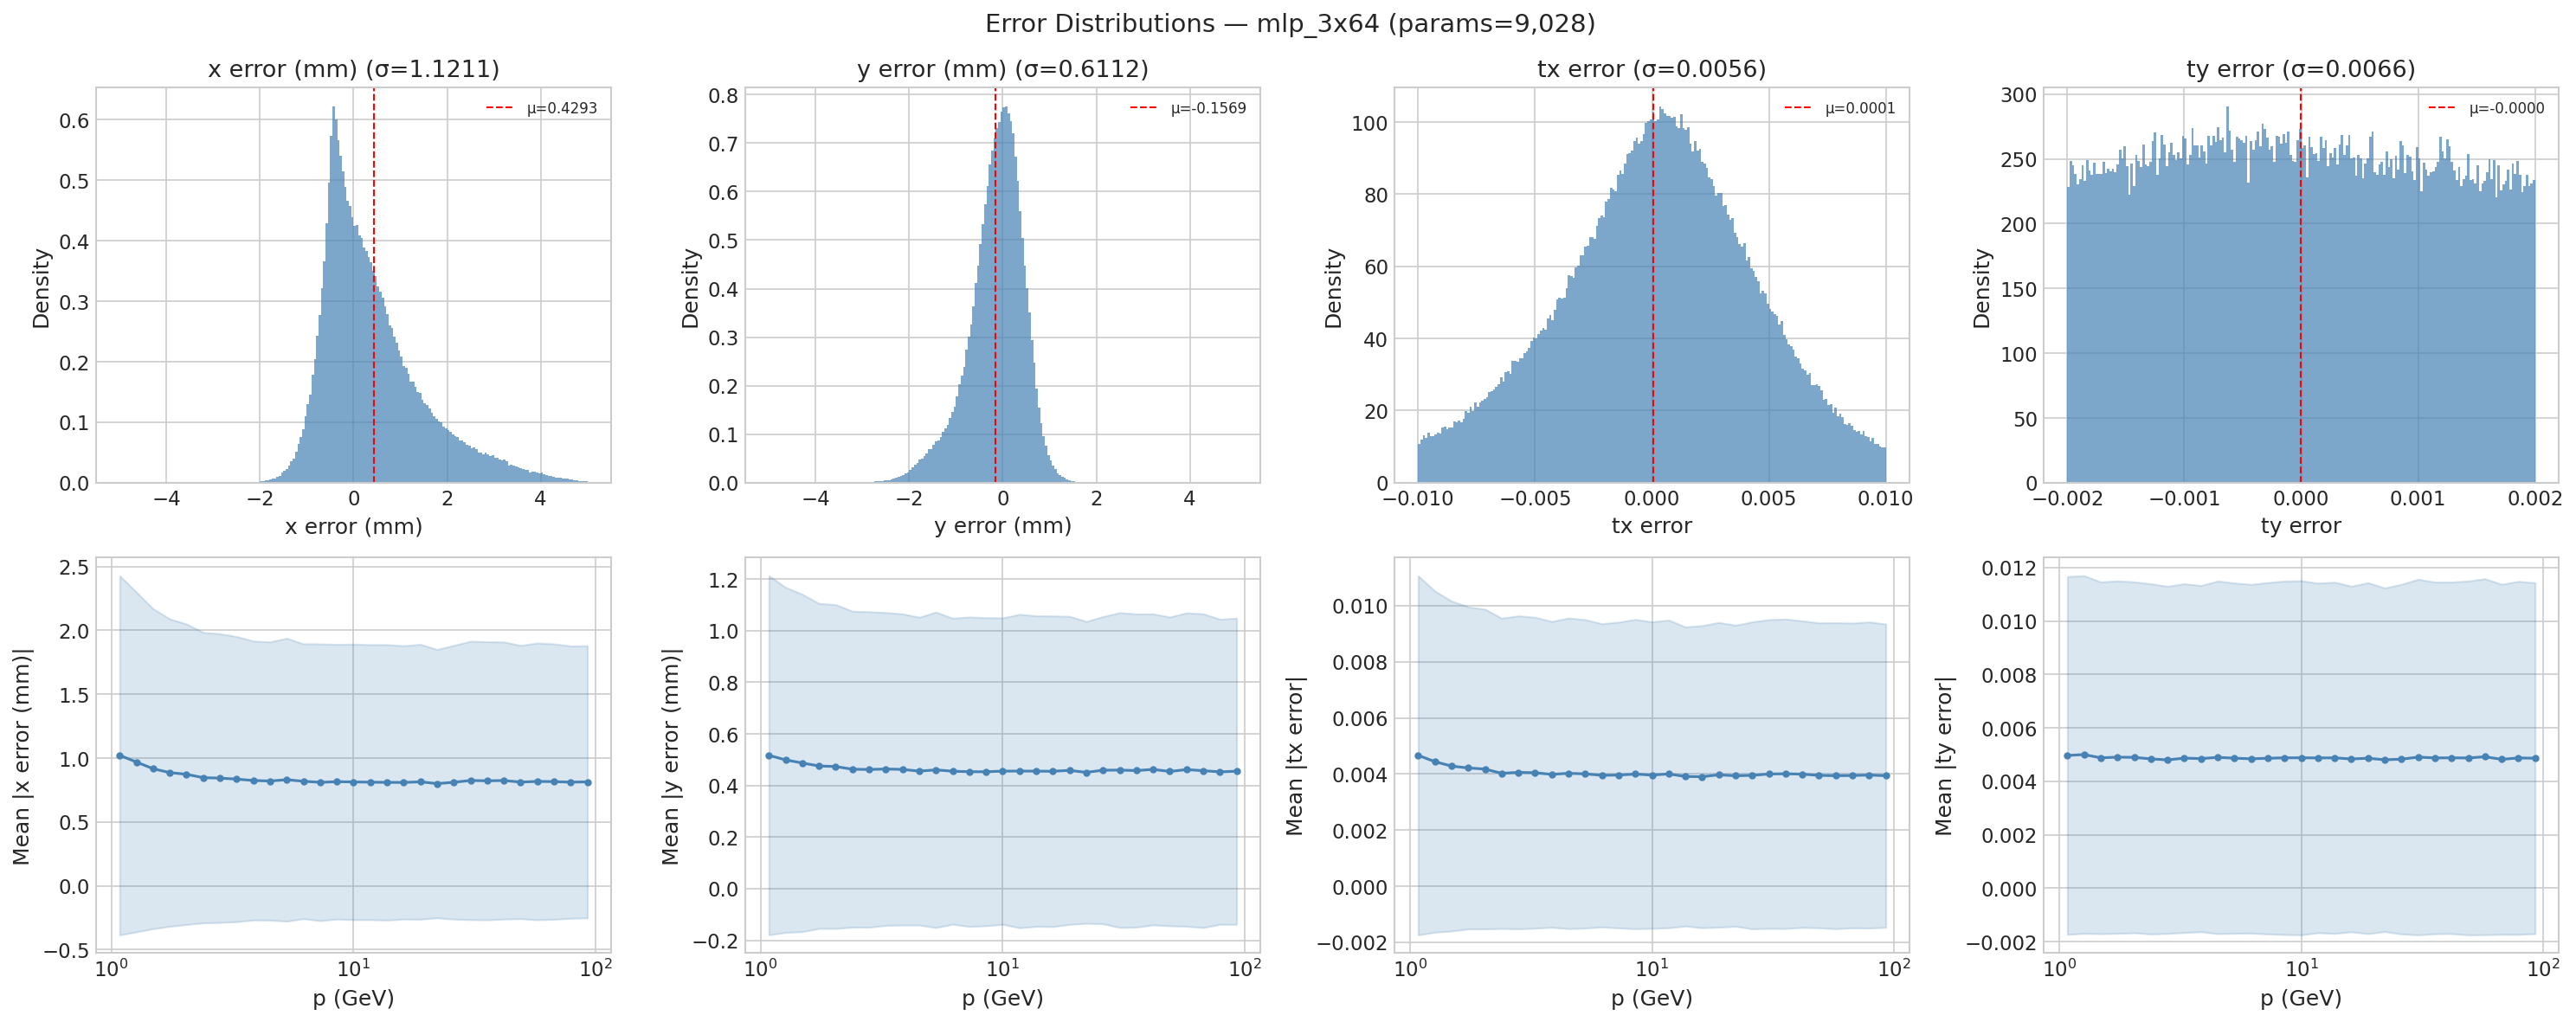
\includegraphics[width=\textwidth]{detailed_error_distributions.png}
\caption{Detailed error distributions for the best model (\texttt{mlp\_3x64}). The position error distribution has a long tail extending to $\sim 10$\,mm for extreme tracks.}
\label{fig:error_dist}
\end{figure}

%=============================================================================
\section{Cost Function Weights for V2 Training}
\label{sec:weights}

\subsection{Residual Target Formulation}
\label{sec:residual}

Following the analysis of Section~\ref{sec:dynamic_range}, V2 training should use \textbf{residual targets} that remove the kinematic term:
\begin{align}
  \delta x &= x' - (x + \tx \cdot \dz) && \text{field-driven position deflection} \\
  \delta y &= y' - (y + \ty \cdot \dz) && \text{field-driven position deflection} \\
  \Delta\tx &= \tx' - \tx && \text{slope change (bending plane)} \\
  \Delta\ty &= \ty' - \ty && \text{slope change (non-bending plane)}
\end{align}

The network then predicts corrections $(\hat{\delta x}, \hat{\delta y}, \widehat{\Delta\tx}, \widehat{\Delta\ty})$ and the full output is reconstructed as:
\begin{equation}
  x' = x + \tx \cdot \dz + \hat{\delta x}, \qquad \tx' = \tx + \widehat{\Delta\tx}, \qquad \text{etc.}
\end{equation}

\subsection{Inverse-Variance Weighting}
\label{sec:inv_var}

With residual targets, the component-wise variances measured on the test set are:

\begin{table}[H]
\centering
\caption{Residual target variances and derived inverse-variance weights. The normalised weights sum to~4 (one per component).}
\label{tab:weights}
\begin{tabular}{@{}l r r r r@{}}
\toprule
Target            & $\sigma_i$  & $\sigma_i^2$      & $1/\sigma_i^2$ & $w_i$ (norm.) \\
\midrule
$\delta x$       & 0.839727  & 0.70514131  & $1.42$                   & 0.0000 \\
$\delta y$       & 0.086769  & 0.00752889  & $1.33 \times 10^{2}$     & 0.0000 \\
$\Delta\tx$      & 0.000189  & 0.00000004  & $2.81 \times 10^{7}$     & 0.0720 \\
$\Delta\ty$      & 0.000026  & 0.00000000  & $1.54 \times 10^{9}$     & 3.9280 \\
\bottomrule
\end{tabular}
\end{table}

The raw inverse-variance weights span 9 orders of magnitude.
After normalisation (weights summing to 4), nearly all weight is assigned to $\Delta\ty$ (3.93) and $\Delta\tx$ (0.07), with position components receiving negligible weight.

\subsection{Practical Weight Prescription}

The pure inverse-variance weights are extreme and would cause the model to entirely ignore position errors.
In practice, several approaches are viable:

\paragraph{Option A: Log-balanced weights.}
Use logarithmically-spaced weights that partially compensate the dynamic range without fully inverting it:
\begin{equation}
  \mathcal{L}_A = \text{MSE}(\delta x) + 10\,\text{MSE}(\delta y) + 10^4\,\text{MSE}(\Delta\tx) + 10^6\,\text{MSE}(\Delta\ty)
  \label{eq:log_weights}
\end{equation}

\paragraph{Option B: Standardised targets.}
Normalise each residual target to unit variance during preprocessing, then use uniform MSE:
\begin{equation}
  \mathcal{L}_B = \text{MSE}\!\left(\frac{\delta x}{\sigma_{\delta x}}\right) + \text{MSE}\!\left(\frac{\delta y}{\sigma_{\delta y}}\right) + \text{MSE}\!\left(\frac{\Delta\tx}{\sigma_{\Delta\tx}}\right) + \text{MSE}\!\left(\frac{\Delta\ty}{\sigma_{\Delta\ty}}\right)
  \label{eq:std_targets}
\end{equation}
This is mathematically equivalent to inverse-variance weighting but numerically better conditioned.

\paragraph{Option C: Tunable $\alpha$-balanced weights.}
Interpolate between uniform and inverse-variance using a parameter $\alpha \in [0, 1]$:
\begin{equation}
  w_i = \sigma_i^{-2\alpha}, \qquad \alpha = 0 \;\text{(uniform)}, \quad \alpha = 1 \;\text{(full inverse-variance)}
  \label{eq:alpha_weights}
\end{equation}

\paragraph{Recommendation.}
We recommend \textbf{Option~B} (standardised targets) for V2.
This is the simplest to implement --- the existing z-score normalisation pipeline already computes per-component means and standard deviations --- and ensures all four components contribute equally to the gradient from the first epoch.
The effective weights are:
\begin{equation}
\boxed{
  w_{\delta x} = \frac{1}{0.8397^2} = 1.42, \quad
  w_{\delta y} = \frac{1}{0.0868^2} = 133, \quad
  w_{\Delta\tx} = \frac{1}{(1.88 \times 10^{-4})^2} = 2.81 \times 10^7, \quad
  w_{\Delta\ty} = \frac{1}{(2.55 \times 10^{-5})^2} = 1.54 \times 10^9
}
\label{eq:final_weights}
\end{equation}

\subsection{Additional Architecture Recommendations}

Based on the V1 analysis, V2 should also incorporate:

\begin{enumerate}[nosep]
  \item \textbf{Residual targets}: Predict field-driven corrections rather than absolute states (Section~\ref{sec:residual}).

  \item \textbf{Multiplicative architecture}: The bending deflection $\Delta\tx \propto \qop$, so use:
  \begin{equation}
    \widehat{\Delta\tx} = (\qop) \cdot g_\theta(\tx, \ty, x, y, z, \dz)
  \end{equation}
  This guarantees $\Delta\tx = 0$ for straight tracks ($\qop = 0$) by construction.

  \item \textbf{$\qop$ skip connection}: Since $\qop$ is an exact invariant ($d(\qop)/dz = 0$), do not predict it --- pass it through unchanged.

  \item \textbf{Small architecture}: The V1 sweep shows that small models ($<$\,35K params) outperform larger ones.
  Start with \texttt{[64, 64, 64]} or \texttt{[256, 128]} and tune from there.
\end{enumerate}

%=============================================================================
\section{Best Model Detailed Performance}
\label{sec:best_model}

Table~\ref{tab:best_detail} summarises the per-component errors for the best V1 model (\texttt{mlp\_3x64}) in both raw and residual space.

\begin{table}[H]
\centering
\caption{Detailed error breakdown for \texttt{mlp\_3x64} (9\,028 parameters).}
\label{tab:best_detail}
\begin{tabular}{@{}l r r r r@{}}
\toprule
Metric & $x$ & $y$ & $\tx$ & $\ty$ \\
\midrule
MAE                 & 0.838 & 0.463 & 0.0040 & 0.0049 \\
Bias                & {$+$0.429} & {$-$0.157} & {$+1 \times 10^{-4}$} & {$-5 \times 10^{-6}$} \\
\midrule
\multicolumn{5}{@{}l}{\textit{Position (combined)}} \\
\midrule
Mean                & \multicolumn{2}{c}{1.017\,mm} & \multicolumn{2}{c}{---} \\
95th percentile     & \multicolumn{2}{c}{2.969\,mm} & \multicolumn{2}{c}{---} \\
99th percentile     & \multicolumn{2}{c}{4.303\,mm} & \multicolumn{2}{c}{---} \\
\midrule
\multicolumn{5}{@{}l}{\textit{Slope (combined)}} \\
\midrule
Mean                & \multicolumn{2}{c}{---} & \multicolumn{2}{c}{0.007058} \\
\bottomrule
\end{tabular}
\end{table}

%=============================================================================
\section{Summary}
\label{sec:summary}

The V1 architecture sweep demonstrates that:

\begin{enumerate}
  \item A 3-layer MLP with only 9K parameters (\texttt{mlp\_3x64}) achieves $\sim\!1.0$\,mm mean position accuracy for LHCb track extrapolation over variable $\dz \in [100, 10\,000]$\,mm, outperforming all larger architectures up to 1M parameters.

  \item The naive MSE loss on raw output states wastes $>$99\% of gradient signal on the kinematic $x + \tx\cdot\dz$ term, leaving slope predictions essentially untrained.

  \item Over-parameterisation (up to 1M parameters) provides no benefit, confirming that model capacity is not the bottleneck --- the loss function is.
\end{enumerate}

For V2 training, we recommend:
\begin{itemize}[nosep]
  \item Residual targets ($\delta x$, $\delta y$, $\Delta\tx$, $\Delta\ty$) to remove the kinematic baseline
  \item Per-component standardisation to unit variance (equivalent to inverse-variance weighting)
  \item Multiplicative $\qop$ gating for slope predictions
  \item A small architecture (\texttt{[64, 64, 64]} or \texttt{[256, 128]})
\end{itemize}

The derived cost function weights and all model binaries have been exported for integration with the Gaudi \texttt{TrackMLPExtrapolator} framework.

\end{document}
